% =====================================================================
% Full report (reconstructed from swd391_topic1.pdf) + Improvement 2 (PoC).
% Generated from a base file plus poc_section.tex (see build_full_report.py).
% Paste the whole result into one main.tex.
% Engine: pdfLaTeX. Packages used are all in a standard TeX Live / Overleaf.
% =====================================================================
\documentclass[11pt,a4paper]{article}

\usepackage[T1]{fontenc}
\usepackage[utf8]{inputenc}
\usepackage{lmodern}
\usepackage[a4paper,margin=2.5cm]{geometry}
\usepackage{amsmath,amssymb}
\usepackage[table]{xcolor}
\usepackage{booktabs,tabularx,array,longtable}
\usepackage{graphicx}
\usepackage{enumitem}
\usepackage{fancyhdr}
\usepackage{tikz}
\usetikzlibrary{positioning,fit,backgrounds,arrows.meta}
\usepackage{algorithm}
\usepackage{algpseudocode}
\usepackage[most]{tcolorbox}
\usepackage[colorlinks=true,linkcolor=blue!50!black,citecolor=blue!50!black,urlcolor=blue!50!black]{hyperref}

\setlength{\parindent}{0pt}
\setlength{\parskip}{6pt}
\setlist{itemsep=2pt,topsep=2pt}

\pagestyle{fancy}
\fancyhf{}
\lhead{SWD391 -- Research Report}
\rhead{Analysis of the SkeltyMLOps paper}
\cfoot{\thepage}
\renewcommand{\headrulewidth}{0.4pt}

\newcolumntype{L}[1]{>{\raggedright\arraybackslash}p{#1}}
\newtcolorbox{callout}[1][]{breakable, colback=blue!4, colframe=blue!50!black, fonttitle=\bfseries, title={#1}}

% Figures of the PoC: shows a placeholder instead of failing when an image is not uploaded yet.
\newcommand{\poctryfig}[2]{\IfFileExists{#2}{\includegraphics[width=#1]{#2}}{\fbox{\parbox{0.8\textwidth}{\centering\small [image \texttt{#2} not uploaded yet]}}}}

\begin{document}

% ---------------------------------------------------------------------
% Title page
% ---------------------------------------------------------------------
\begin{titlepage}
\thispagestyle{empty}
\centering
{\large FPT UNIVERSITY -- HO CHI MINH CITY CAMPUS\par}
\vspace{0.3cm}
{\large SWD391 -- Software Architecture and Design\par}
\vspace{1.2cm}
{\Large\bfseries RESEARCH REPORT\par}
\vspace{0.8cm}
{\huge\bfseries Orchestrating Collaborative MLOps:\\[4pt] An Analysis of the SkeltyMLOps Reference Architecture\par}
\vspace{1.2cm}
{\bfseries Paper under study:}\\[3pt]
C.~Daoud, D.~Azar, C.~Urtado, S.~Vauttier, ``A reference architecture for an orchestrated collaborative MLOps: A ground-up design from literature combining human and LLM expertise,'' \emph{Future Generation Computer Systems}, vol.~185, 108700, 2026.\\
doi: 10.1016/j.future.2026.108700
\vspace{1.2cm}

{\bfseries Group 2}\\[6pt]
\begin{tabular}{@{}cll@{}}
\toprule
No. & Full name & Student ID \\
\midrule
1 & Chung Quoc Huy & SE194569 \\
2 & Luong Gia Luan & SE192603 \\
3 & Vu Nguyen Duc Huy & SE194089 \\
4 & Le Hoang Huy & SE192981 \\
5 & Trinh Nhat Quang & SE192966 \\
\bottomrule
\end{tabular}
\vfill
Instructor: VuLNS\\[4pt]
Ho Chi Minh City, September 2026
\end{titlepage}

% ---------------------------------------------------------------------
% Abstract and contents
% ---------------------------------------------------------------------
\begin{abstract}
This report analyses the paper by Daoud et al.~\cite{daoud2026}, which proposes SkeltyMLOps, a modular reference software architecture for orchestrated collaborative Machine Learning Operations (MLOps). The paper follows a two-phase design. In Phase~1, a systematic literature review of 53 peer-reviewed papers extracts 16 actor names and 402 activity statements, which are consolidated by human experts assisted by a Large Language Model (LLM) into five MLOps dimensions (Plan, Data, Model, Software, Ops) and 38 activities. In Phase~2, five published MLOps architectures are scored against the resulting 44-element scope to expose recurring coordination gaps, and SkeltyMLOps is designed from the ground up, with an MLOps Process Orchestrator that executes versioned coordination contracts over tickets and events. Following the assignment criteria, we present the paper's introduction, research questions, literature review, hypotheses, methods, data sources and results, and we close with our own critical assessment. We also recompute the paper's coverage metrics from its raw scoring matrix and find them consistent.
We complement the assessment with two improvements: we score SkeltyMLOps and three other architectures on six criteria (Improvement 1), and we instantiate the paper's data-drift scenario as a proof of concept on a Kubernetes cluster and report one end-to-end run (Improvement 2).
\end{abstract}

\tableofcontents
\newpage

% =====================================================================
\section{Short Introduction}\label{sec:intro}

\subsection{The paper at a glance}

\begin{table}[h]
\centering
\caption{Bibliographic overview of the paper under study.}
\small
\begin{tabularx}{\textwidth}{@{}L{3.2cm}X@{}}
\toprule
Title & A reference architecture for an orchestrated collaborative MLOps: A ground-up design from literature combining human and LLM expertise \\
Authors & Charbel Daoud, Danielle Azar, Christelle Urtado, Sylvain Vauttier \\
Affiliations & SyCoIA, IMT Mines Al\`es (France); Dept.\ of Computer Science \& Mathematics, Lebanese American University (Lebanon) \\
Venue & Future Generation Computer Systems (Elsevier), vol.~185, article 108700, 2026 -- special issue ``MLOps'' \\
Timeline & Received 31 March 2026; revised 1 July 2026; accepted 2 July 2026; online 11 July 2026 \\
Access & Open access (CC BY 4.0); DOI 10.1016/j.future.2026.108700 \\
Relation to prior work & Extended version of a workshop paper presented at MLOps@ECAI 2025~\cite{daoud2025} \\
Research type & Systematic literature review + design-oriented research (reference architecture) \\
Replication package & Raw extraction data, prompts, LLM configurations, scripts and outputs on Zenodo~\cite{zenodo} \\
Funding & R\'egion Occitanie (PLANETS project); French National Research Agency (AdaptiveMLOps, ANR-24-IAS2-0004) \\
\bottomrule
\end{tabularx}
\end{table}

\subsection{Background and motivation}

\textbf{ML-powered software degrades after deployment.}
Machine learning (ML) is increasingly embedded in software, and the value of ML-powered software depends not only on model accuracy but on the ability to ship, operate and evolve all of its artefacts -- data, models and code -- reliably over time. Once deployed, models face changing data distributions (data drift), shifting user behaviour and evolving operational constraints, so performance may degrade without explicit failures. Sculley et al.~\cite{sculley2015} showed that these dynamics accumulate hidden technical debt: maintenance costs and operational risks grow unless the software supports monitoring, reproducibility and disciplined change management. MLOps emerged by borrowing and adapting DevOps practices so that operationalisation covers AI models and data, not only code.

\textbf{A persistent engineering and coordination gap.}
Despite the growing number of MLOps tools and platforms, practitioners still face a gap: MLOps solutions are often assembled from heterogeneous tools whose integration and governance are complex, costly and hard to adapt. The authors argue that such integration decisions are really coordination decisions: specialised actors (data, model, software and operations engineers) must agree on ownership boundaries and handoff protocols. Breakdowns typically occur at cross-actor boundaries, where responsibilities are ambiguous and dependencies between data, models and software are neither explicit nor managed. In addition, the field lacks a commonly adopted definition of MLOps: studies use different terminology for its actors and activities, which makes it hard to design an architecture on a solid conceptual basis.

\textbf{The proposal: SkeltyMLOps.}
To address this gap, the paper proposes SkeltyMLOps, a reference software architecture -- i.e., a reusable template of structures, elements and relationships for building software in a given domain -- for orchestrated collaborative MLOps. The architecture is not designed ad hoc: it is derived ``from the ground up'' from a systematic literature review whose extracted terms are clustered and normalised by human experts assisted by LLMs. Its distinguishing feature is that orchestration and cross-actor coordination are placed at the core of the architecture, through an MLOps Process Orchestrator (MPO) and explicit coordination contracts.

\subsection{Research objective and contributions}

The paper's stated objective is to fill the absence of ``an accepted, accessible, and modular reference architecture for MLOps'' by designing one that promotes collaboration among the diverse actors involved. The authors list four contributions:
\begin{enumerate}[label=\textbf{C\arabic*.}]
  \item a structured characterisation of MLOps from the literature, consolidating scattered terminology into a clear set of actors, activities and dimensions;
  \item a consolidation process that combines human and LLM expertise to normalise and cluster the extracted actors and activities;
  \item SkeltyMLOps, a modular reference architecture for orchestrated MLOps, built around tickets, handoffs and coordination contracts;
  \item a comparative coverage analysis against existing MLOps architectures, which the authors present as assessing how far the proposed architecture captures the identified activities and key collaboration concerns (see the clarification in Section~\ref{sec:methods} and point W1 in Section~\ref{sec:assessment}).
\end{enumerate}
According to the abstract, the originality of the work is twofold: (1) the careful knowledge-gathering process that grounds the architecture, and (2) the central role given to orchestration and coordination.

\subsection{Organisation of this report}

Table~\ref{tab:org} maps the assignment criteria to the sections of this report.

\begin{table}[h]
\centering
\caption{Mapping between the assignment criteria and this report.}\label{tab:org}
\small
\begin{tabularx}{\textwidth}{@{}L{3.2cm}XL{1.4cm}@{}}
\toprule
Criterion & What is covered & Section \\
\midrule
Short Intro & Paper metadata, context, objective, contributions & \ref{sec:intro} \\
Research Question & RQ1--RQ4, rationale, RQ-to-method-to-result mapping & \ref{sec:rq} \\
Literature Review & DevOps$\rightarrow$MLOps background, prior secondary studies, prior architectures, research gap & \ref{sec:lit} \\
Hypothesis & Why no formal hypothesis; implicit hypotheses and design propositions & \ref{sec:hyp} \\
Methods & Two-phase design; Methods A--D; threats to validity & \ref{sec:methods} \\
Data Source & Literature corpus, extracted data, LLM experiment data, baseline architectures & \ref{sec:data} \\
Result of the paper & Results for RQ1--RQ4, gap analysis, limitations and future work & \ref{sec:results} \\
(Additional) & Our critical assessment and verification & \ref{sec:assessment} \\
(Additional) & Improvement 1: scoring of four architectures on six criteria & \ref{sec:scoring} \\
(Additional) & Improvement 2: proof-of-concept instantiation of the data-drift scenario & \ref{sec:poc} \\
\bottomrule
\end{tabularx}
\end{table}

% =====================================================================
\section{Research Questions}\label{sec:rq}

The study is organised in two phases, and four research questions (RQs) guide it. Phase~1 (Literature Analysis Review) answers RQ1--RQ3; Phase~2 (Orchestration and Collaboration) answers RQ4 using the results of Phase~1 as its foundation.

\begin{callout}[Research questions of the paper]
\textbf{Phase 1 -- Literature Analysis Review}
\begin{itemize}
  \item \textbf{RQ1:} Who are the main actors involved in MLOps?
  \item \textbf{RQ2:} What are the dimensions of MLOps?
  \item \textbf{RQ3:} What are the activities that constitute MLOps processes?
\end{itemize}
\textbf{Phase 2 -- Orchestration and Collaboration}
\begin{itemize}
  \item \textbf{RQ4:} How can a modular MLOps reference architecture be designed to integrate the activities identified in RQ3 and to facilitate collaboration among the actors identified in RQ1?
\end{itemize}
\end{callout}

\subsection{Rationale of each question}

\textbf{RQ1 -- Actors.}
A collaboration-centred architecture must first know who collaborates. The literature names the same responsibilities differently (e.g., the model-building actor is called Data Scientist in some papers and ML Engineer/Developer in others), so the actors must be identified and consolidated before responsibilities can be assigned to architectural modules.

\textbf{RQ2 -- Dimensions.}
A dimension is ``a distinct functional area that groups related actors and responsibilities''. DevOps has only two (Dev and Ops), which does not reflect data- and model-centric work. The dimensions give the architecture its top-level decomposition.

\textbf{RQ3 -- Activities.}
Activities define what an MLOps process must support. The consolidated list is also reused as the scope for the coverage analysis in Phase~2.

\textbf{RQ4 -- Architecture.}
This is a design question: how to turn the evidence of RQ1--RQ3 into a modular architecture in which activities are integrated and cross-actor collaboration is explicit.

\subsection{From questions to answers}

The questions form a progressive chain: who is involved (RQ1) $\rightarrow$ how they group into functional areas (RQ2) $\rightarrow$ what they do (RQ3) $\rightarrow$ how an architecture should integrate all of this and coordinate them (RQ4). Table~\ref{tab:rq} links each RQ to the method used and the main answer (details in Sections~\ref{sec:methods} and~\ref{sec:results}).

\begin{table}[h]
\centering
\caption{Research questions, methods, paper sections and key answers.}\label{tab:rq}
\small
\begin{tabularx}{\textwidth}{@{}L{0.9cm}L{2.6cm}L{1.6cm}X@{}}
\toprule
RQ & Method(s) & Paper \S & Key answer \\
\midrule
RQ1 & A (SLR, manual extraction) + B (LLM-assisted clustering) & \S3, \S4.1 & 16 extracted actor names consolidated into 5 clusters, each with a leading actor: Product Owner, Data Engineer, Model Engineer, Software Engineer, Operations Engineer. \\
RQ2 & B & \S4.1, \S4.5 & 5 dimensions -- Plan, Data, Model, Software, Ops -- forming a ``revisited MLOps loop'' that splits the Dev side of DevOps into Data, Model and Software. \\
RQ3 & A + B (5-step consolidation) & \S4.2--4.4 & 402 activity statements consolidated into 38 activities: 17 shared with DevOps, 21 ML-specific. \\
RQ4 & C (gap analysis) + D (ground-up design) & \S5 & SkeltyMLOps: 5 packages, 11 components (7 of which implement the 38 activities), and an MPO that executes coordination contracts over tickets and events. \\
\bottomrule
\end{tabularx}
\end{table}

% =====================================================================
\section{Literature Review}\label{sec:lit}

\subsection{From DevOps to MLOps}

DevOps bridges software development and operations to shorten release cycles by formalising automation and fast feedback loops. It is commonly drawn as an infinite loop that links development activities (Plan, Code, Build, Test) with operational activities (Release, Deploy, Operate, Monitor), where production monitoring feeds back into requirements, planning and implementation. At a high level, this loop spans two dimensions: Dev and Ops.

In ML-powered software, the loop must absorb additional sources of change: after deployment, the data distribution may change, features may become outdated and model performance may degrade. Foundational work on ML technical debt~\cite{sculley2015} argues that these dynamics create hidden costs unless the software supports monitoring, reproducibility and disciplined change management. MLOps therefore extends DevOps by redefining development and operations around code, data and models, with mechanisms such as data and model versioning, experiment tracking, model registries, continuous evaluation, and retraining and redeployment when appropriate.

Although many tools and platform stacks exist, empirical and secondary studies report recurring architectural problems: the absence of unified architectural guidance, the complexity of integrating heterogeneous components, and the limited modularity of many commercial solutions. Studies of open-source practice further indicate that accessible and reusable reference architectures remain scarce.

\subsection{Prior secondary studies}

Several secondary studies have surveyed the MLOps field. Table~\ref{tab:secondary} (reproduced from Table~1 of the paper) compares their scope along four concerns: actors, activities, coordination and architecture.
\begin{itemize}
  \item Kreuzberger et al.~\cite{kreuzberger2023} combine a literature review, a tool review and expert interviews to define MLOps principles, components and actors, and propose an overview architecture.
  \item Najafabadi et al.~\cite{najafabadi2024} map MLOps architectures through a systematic mapping study and synthesise 35 architectural components.
  \item Eken et al.~\cite{eken2025} conduct a multivocal review (including grey literature) covering practices, actors, activities, challenges and open issues.
  \item Wo\'zniak et al.~\cite{wozniak2025} review MLOps components, tools and process steps.
\end{itemize}

\begin{table}[h]
\centering
\caption{Scope of prior secondary studies ($\checkmark$ = primary concern; $\circ$ = partial; -- = not addressed). Adapted from Table~1 of~\cite{daoud2026}.}\label{tab:secondary}
\small
\begin{tabular}{@{}lrlcccc@{}}
\toprule
Study & \# sources & Type & Actors & Activities & Coord. & Arch. \\
\midrule
Kreuzberger et al. (2023)~\cite{kreuzberger2023} & 27 & Mixed method & $\checkmark$ & $\checkmark$ & $\circ$ & $\checkmark$ \\
Najafabadi et al. (2024)~\cite{najafabadi2024} & 43 & Systematic mapping & -- & -- & -- & $\checkmark$ \\
Eken et al. (2025)~\cite{eken2025} & 198 & Multivocal review & $\checkmark$ & $\checkmark$ & $\circ$ & -- \\
Wo\'zniak et al. (2025)~\cite{wozniak2025} & 41 & SLR & -- & $\checkmark$ & -- & $\checkmark$ \\
Daoud et al. (2026) (this paper) & 53 & SLR & $\checkmark$ & $\checkmark$ & $\checkmark$ & $\checkmark$ \\
\bottomrule
\end{tabular}
\end{table}

Although some of these studies report actors or activities, none performs a systematic extraction and consolidation that normalises the heterogeneous terminology into a unified characterisation linking actors to their activities. Moreover, coordination across actors -- ownership boundaries, handoff specifications and governance mechanisms -- is not treated as a primary concern in any of them.

\subsection{Existing MLOps architectures}

The paper positions its architecture against representative MLOps architectures that cover four complementary perspectives:
\begin{itemize}
  \item specialised operational architectures, e.g., Rodrigues et al.~\cite{rodrigues2025} for near real-time distributed stream learning;
  \item tool-oriented, open-source blueprints, e.g., Burgue\~no-Romero et al.~\cite{burgueno2025};
  \item industry-driven reference architectures, e.g., Kumara et al.~\cite{kumara2025}, derived from industrial requirements and pipeline patterns;
  \item survey-based overviews, e.g., Najafabadi et al.~\cite{najafabadi2024} and Kreuzberger et al.~\cite{kreuzberger2023}.
\end{itemize}
These works clarify what MLOps software generally contains and which stages are commonly distinguished. However, they give limited guidance on how the actors coordinate their work across ownership boundaries, approvals, handoffs and runtime feedback loops.

\subsection{Research gap}

\begin{callout}[Research gap identified by the paper]
\begin{description}[leftmargin=1.4cm,style=nextline]
  \item[G1.] \textbf{Fragmented terminology} -- there is no universally adopted definition of MLOps; actor and activity names vary across studies.
  \item[G2.] \textbf{Missing actor--activity mapping} -- no study jointly extracts and consolidates actors and activities from the literature.
  \item[G3.] \textbf{Implicit coordination} -- handoffs, ownership and governance are treated as by-products of tools or processes rather than as primary architectural concerns.
  \item[G4.] \textbf{Scarce reference architectures} -- accessible, modular and reusable reference architectures for MLOps are still missing.
\end{description}
\end{callout}

G1 and G2 motivate RQ1--RQ3; G3 and G4 motivate RQ4.

% =====================================================================
\section{Hypothesis}\label{sec:hyp}

\subsection{Why the paper has no formal hypothesis}

The study does not follow a quantitative hypothesis-testing design. Instead of causal hypotheses (e.g., ``H1: X positively affects Y''), it is organised around four research questions that guide an exploratory, literature-grounded investigation (RQ1--RQ3) and a design-oriented contribution (RQ4). This is consistent with its goal: characterising a domain and constructing an artefact (a reference architecture), rather than testing a relationship between variables.

Nevertheless, several hypothesis-like claims can be identified. Two are tested empirically in the LLM sub-study (Methods B), and two are propositions that the paper argues for without a statistical test.

\subsection{Implicit hypotheses tested in the LLM sub-study}

\textbf{H1 -- LLM configurations differ.}
Different LLM configurations (provider, temperature and reasoning mode) yield measurably different levels of coverage, validity and stability when clustering and labelling MLOps actors. The hypothesis is examined by running 13 configurations from OpenAI, Anthropic, Google and DeepSeek ten times each on the same clustering task and comparing four indicators (coverage, invalid items, duplicate assignments, and mean/standard deviation of the number of dimensions). The results support it: coverage ranges from 98.75\% to 100\%, mean duplicate assignments from 0 to 4 per run, and the standard deviation of the number of dimensions from 0.00 to 2.96. Gemini 2.5 Flash at temperature 0 is the only configuration that combines full coverage, zero invalid items, zero duplicates and a perfectly stable dimension count, and is therefore selected as the ``champion''.

\textbf{H2 -- Retrieval helps.}
Adding Retrieval-Augmented Generation (RAG) -- giving the model the full PDF papers -- improves consolidation quality for the champion configuration. Tested by comparing RAG and no-RAG settings under the same prompt and parameters. The hypothesis is not supported: both reach 100\% coverage, but the RAG configuration introduces an invalid actor (``ML Architect'') that is not in the extracted list. The no-RAG configuration is retained.

\subsection{Propositions argued without statistical testing}

\textbf{P1 -- MLOps extends a DevOps backbone (descriptive).}
MLOps builds on a software-delivery backbone inherited from DevOps while adding explicit activities for evolving data and model artefacts. Supported descriptively by the consolidated activity list: 17 of the 38 activities also appear in DevOps, and several of the most frequently reported activities (e.g., Preprocess Data, Train Model, Evaluate \& Test Model) are ML-specific.

\textbf{P2 -- Orchestration-centred design is reusable guidance (design proposition for RQ4).}
In its conclusion the paper claims that ``an actor-aligned, orchestration-centered decomposition can serve as reusable architectural guidance for collaborative MLOps settings while remaining independent of a specific tool stack.'' This proposition is supported by (i) the traceable derivation of the architecture from the Phase~1 evidence, (ii) the gap analysis of five existing architectures and (iii) an illustrative data-drift scenario. It is not empirically tested: SkeltyMLOps has not been instantiated in a production setting, and it is not itself scored in the coverage analysis.

\begin{table}[h]
\centering
\caption{Summary of implicit hypotheses and propositions.}
\small
\begin{tabularx}{\textwidth}{@{}L{0.9cm}XL{3.4cm}L{3.2cm}@{}}
\toprule
ID & Statement & How examined & Status \\
\midrule
H1 & LLM configurations differ in coverage, validity and stability & 13 configurations $\times$ 10 runs, 4 indicators & Supported $\rightarrow$ Gemini 2.5 Flash, $T=0$ \\
H2 & RAG improves consolidation quality & RAG vs.\ no-RAG on the champion & Not supported $\rightarrow$ no-RAG kept \\
P1 & MLOps = DevOps backbone + ML-specific activities & DevOps-overlap flag on the 38 activities & Supported descriptively (17/38 shared) \\
P2 & Actor-aligned, orchestration-centred design is reusable guidance & Derivation, gap analysis, illustrative scenario & Argued and illustrated, not empirically tested \\
\bottomrule
\end{tabularx}
\end{table}

% =====================================================================
\section{Methods Used in the Paper}\label{sec:methods}

\subsection{Overall research design}

The paper uses a two-phase, mixed-method design in which the output of Phase~1 becomes the input of Phase~2 (Figure~\ref{fig:design}). Phase~1 is a qualitative, evidence-based synthesis of the literature; Phase~2 is constructive (design-oriented). The chain is sequential and traceable: literature $\rightarrow$ extracted evidence $\rightarrow$ consolidated scope (44 elements) $\rightarrow$ gap analysis of existing architectures $\rightarrow$ ground-up architecture design.

\begin{figure}[h]
\centering
\resizebox{\textwidth}{!}{%
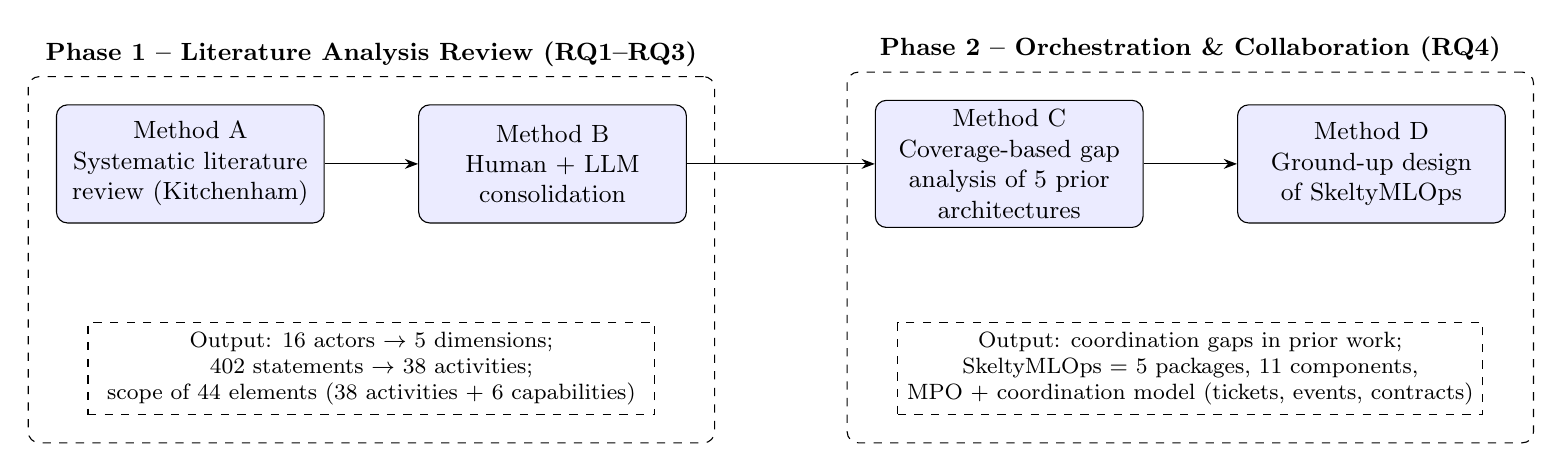
\begin{tikzpicture}[
  meth/.style={draw, rounded corners, align=center, minimum width=3.4cm, minimum height=1.5cm, fill=blue!8, font=\small},
  outp/.style={draw, dashed, align=center, minimum width=7.2cm, minimum height=1.1cm, font=\footnotesize},
  >=Stealth]
\node[meth] (A) at (0,0)    {Method A\\Systematic literature\\review (Kitchenham)};
\node[meth] (B) at (4.6,0)  {Method B\\Human + LLM\\consolidation};
\node[meth] (C) at (10.4,0) {Method C\\Coverage-based gap\\analysis of 5 prior\\architectures};
\node[meth] (D) at (15,0)   {Method D\\Ground-up design\\of SkeltyMLOps};
\draw[->] (A) -- (B);
\draw[->] (B) -- (C);
\draw[->] (C) -- (D);
\node[outp] (o1) at (2.3,-2.6)  {Output: 16 actors $\rightarrow$ 5 dimensions;\\402 statements $\rightarrow$ 38 activities;\\scope of 44 elements (38 activities + 6 capabilities)};
\node[outp] (o2) at (12.7,-2.6) {Output: coordination gaps in prior work;\\SkeltyMLOps = 5 packages, 11 components,\\MPO + coordination model (tickets, events, contracts)};
\begin{scope}[on background layer]
  \node[draw, dashed, rounded corners, inner sep=10pt, fit=(A)(B)(o1), label={[font=\small\bfseries]above:Phase 1 -- Literature Analysis Review (RQ1--RQ3)}] {};
  \node[draw, dashed, rounded corners, inner sep=10pt, fit=(C)(D)(o2), label={[font=\small\bfseries]above:Phase 2 -- Orchestration \& Collaboration (RQ4)}] {};
\end{scope}
\end{tikzpicture}}
\caption{Two-phase research design (adapted from Fig.~2 of~\cite{daoud2026}; the gap-analysis step of Phase~2, described in \S5.2--5.4 of the paper, is made explicit here).}\label{fig:design}
\end{figure}

\begin{callout}[Note on the order of Phase 2]
In the paper, the comparison of existing architectures (\S5.2--5.4) comes before the design of SkeltyMLOps (\S5.5--5.9). The comparison therefore works as a gap analysis that motivates the design, not as a post-hoc benchmark of SkeltyMLOps against other architectures.
\end{callout}

\subsection{Phase 1 -- Method A: Systematic literature review}

The SLR follows Kitchenham's guidelines for systematic reviews in software engineering~\cite{kitchenham2007}.

\textbf{A1. Choice of data source.} Google Scholar is used as a meta-indexer: a single query covers IEEE, ACM, Springer, Elsevier, MDPI and other publishers without adapting the query to each database.

\textbf{A2. Search string.} Terms are derived from RQ1--RQ3 (MLOps, actors, activities, processes, architecture) and refined with synonyms. The \texttt{allintitle:} operator targets papers that explicitly position themselves in the MLOps space (precision over recall); its limitations are compensated by screening and snowballing. The exact string is given in Section~\ref{sec:data}.

\textbf{A3. Calibration.} Two authors independently screen the same 10 pilot papers and resolve disagreements in a consensus meeting to finalise the interpretation of the criteria and coding rules.

\textbf{A4. Screening with inclusion/exclusion criteria.} A paper is included if it explicitly reports at least one extractable artefact: (i) a set of MLOps actors, (ii) a process depiction (e.g., a process figure), or (iii) an explicit enumeration of MLOps activities. It is excluded if it is non-English, has no accessible full text, is not peer-reviewed, or is only available through inaccessible subscriptions.

\textbf{A5. Snowballing.} Backward (cited) and forward (citing) snowballing mitigates the title-based query; new papers are filtered with the same criteria.

\textbf{A6. Manual extraction.} For each paper, the authors record bibliographic metadata, the actors mentioned (RQ1) and the activities reported in text or process figures (RQ3). A content-analysis approach with predefined categories is used, manually and independently by two authors; disagreements are resolved by consensus.

\textbf{A7. Inter-rater agreement.} Pre-consensus agreement is measured with Cohen's $\kappa$ on a binary (present/absent) matrix: after synonym normalisation, the unique items across all papers form a reference list (38 actor names and 58 activity types), and each rater's extraction is coded per (paper, item) pair. Results: $\kappa = 0.808$ for actors and $\kappa = 0.780$ for activities, i.e., ``substantial agreement'' on the Landis--Koch scale~\cite{landis1977}.

\subsection{Phase 1 -- Method B: Human and LLM consolidation}

\textbf{Why a consolidation step is needed.}
The raw extraction is highly heterogeneous: actor names vary in naming and granularity (near-synonyms, overloaded names), some papers separate model-centric from software-centric actors, business actors are rarely visible (explicit in only 7 of the 38 papers contributing to RQ1), and the 402 activity statements range from fine-grained implementation steps to coarse process stages. Consolidating this by hand across papers would be slow and hard to reproduce, since different researchers may produce different groupings.

\textbf{Principles for using LLMs.}
\begin{itemize}
  \item LLMs are not used for extraction, which is fully manual (Method A). They are used only to (i) cluster artefacts with similar meaning despite lexical variation and (ii) propose names for clusters.
  \item The LLM is an analysis aid, not a decision maker: all outputs are provisional and are revised or rejected by human experts (unsupported groupings, misleading names, overly general categories) through negotiated agreement.
  \item Every override is recorded in a Human Modification Log (modification type, proposed item, final item, justification), published in the replication package.
  \item All prompts share one structure: objective, artefact under analysis, constraints and output schema.
\end{itemize}

\textbf{B1 -- Controlled experiment to select the LLM configuration.}
Thirteen configurations from four providers are compared (Table~\ref{tab:llmconf}). Temperatures 0 and 0.7 are used where available; temperature 1 is also used for Claude Sonnet 4.6 and Gemini 2.5 Flash to activate their reasoning mode; o3, o4-mini and DeepSeek Reasoner only allow their default temperature.

\begin{table}[h]
\centering
\caption{The 13 LLM configurations compared (from Table~3 of~\cite{daoud2026}).}\label{tab:llmconf}
\small
\begin{tabular}{@{}llll@{}}
\toprule
Provider & Model & Mode & Temperature(s) \\
\midrule
Anthropic & Claude Sonnet 4.6 & Chat / Reasoning & 0, 0.7 / 1 \\
DeepSeek & DeepSeek Chat & Chat & 0, 0.7 \\
DeepSeek & DeepSeek Reasoner & Reasoning & Default \\
Google & Gemini 2.5 Flash & Chat / Reasoning & 0, 0.7 / 1 \\
OpenAI & GPT-4o & Chat & 0, 0.7 \\
OpenAI & o3 & Reasoning & Default \\
OpenAI & o4-mini & Reasoning & Default \\
\bottomrule
\end{tabular}
\end{table}

Each configuration receives the same task (propose dimensions from the 16 actors, assign actors to dimensions, propose a leading actor per dimension) and is run 10 times. The indicators are:
\begin{itemize}
  \item \textbf{Coverage (\%)} -- share of the extracted actors that appear in the output;
  \item \textbf{Invalid items per run} -- mean number of items outside the extracted actor list;
  \item \textbf{Duplicate assignments per run} -- mean number of actors assigned to more than one dimension;
  \item \textbf{Mean and standard deviation of the number of dimensions} -- structural stability across runs;
\end{itemize}
plus compliance with the required output schema. Since almost all configurations reach full coverage, the selection is driven by correctness and stability: zero duplicates, low variability of the dimension count and consistent schema output.

\textbf{B2 -- RAG vs.\ no-RAG.}
For the champion, a RAG setting (extracted artefacts and full PDF papers) is compared with a no-RAG setting (prompt and extracted artefacts only), with identical prompt and parameters. This isolates the effect of external grounding.

\textbf{B3 -- Five-step consolidation of activities.}
(1)~\emph{Assignment to validated dimensions} -- the champion LLM classifies each of the 402 statements into one of the validated dimensions; humans correct misplaced assignments.
(2)~\emph{Dimension-specific clustering} -- activities are clustered within each dimension to avoid merging activities that look similar but belong to different operational contexts.
(3)~\emph{Redundancy reduction and normalisation} -- a dedicated prompt groups similar activities, avoids merging distinct tasks and produces concise, stable labels.
(4)~\emph{Expert review and final merging} -- humans remove residual overlap, refine labels and check that each activity fits the responsibility boundaries of its dimension.
(5)~\emph{Final consolidation with metadata} -- each activity receives a short description, a flag indicating whether it also appears in DevOps (assessed by human experts) and its frequency in the corpus.

\subsection{Phase 2 -- Method C: Coverage-based gap analysis of existing architectures}

\textbf{Baselines.}
Five published architectures are chosen to represent distinct contributions: an architecture for near real-time stream learning operations (Rodrigues et al.~\cite{rodrigues2025}), an open-source architecture blueprint (Burgue\~no-Romero et al.~\cite{burgueno2025}), an industry-driven reference architecture (Kumara et al.~\cite{kumara2025}), an architecture synthesised from a mapping study (Najafabadi et al.~\cite{najafabadi2024}) and a survey-based overview architecture (Kreuzberger et al.~\cite{kreuzberger2023}).

\textbf{Scope of 44 elements.}
Each baseline is scored against the 38 consolidated activities of Phase~1 plus six cross-cutting capabilities: (i) explicit actor-to-responsibility mapping, (ii) cross-actor handoff specification, (iii) traceability across data, model, code and operational artefacts, (iv) governance gates, (v) feedback loops (monitor $\rightarrow$ decision $\rightarrow$ action) and (vi) software versioning.

\textbf{Scoring rubric.}
Each (baseline, element) pair receives a score $s \in \{0, 1, 2\}$:
\begin{itemize}
  \item \textbf{Absent (0)} -- the element is neither described nor supported, and cannot reasonably be grounded in the text or figures without speculation;
  \item \textbf{Partial (1)} -- the element is mentioned or implied, but no concrete mechanism is specified (named module, process activity or actor ownership);
  \item \textbf{Explicit (2)} -- the element is supported by an identifiable architectural element and/or a clearly described process activity with stated responsibilities and exchanged artefacts.
\end{itemize}

\textbf{Procedure.}
Two authors score all baselines independently by mapping components in the architecture figures to elements, confirming scope and responsibilities in the descriptions, and running targeted keyword searches (registry, versioning, CI/CD, monitoring, drift, pipeline, feature store, staging). A rationale (section or figure reference plus justification) is recorded for every partial or explicit score. Pre-consensus agreement is measured with a quadratically weighted Cohen's kappa, $\kappa_w = 0.743$ (substantial), after which disagreements are resolved in a consensus meeting.

\textbf{Metrics.}
With $s_i$ the score of element $i$ and $N = 44$:
\[
\text{Total coverage} = \frac{\sum_{i=1}^{N} s_i}{2N}, \qquad
\text{Binary coverage} = \frac{|\{i : s_i \geq 1\}|}{N}, \qquad
\text{Strong coverage} = \frac{|\{i : s_i = 2\}|}{N}.
\]
Binary coverage measures breadth (whether an element is present at all) and strong coverage measures depth (whether it is explicit).

\begin{callout}[Important clarification]
The authors state that this assessment ``is not interpreted as a quality ranking but rather as a structured comparison of explicitness with respect to a fixed scope derived from the literature.'' Only the five baselines are scored: Tables~7 and~8 of the paper contain no column or row for SkeltyMLOps.
\end{callout}

\subsection{Phase 2 -- Method D: Ground-up architecture design}

A reference architecture is a reusable blueprint that captures essential design principles, structural decomposition and interface-level guidance for a domain, allowing several concrete instantiations. SkeltyMLOps is derived from the Phase~1 results through explicit design rules:

\textbf{D1. Dimension $\rightarrow$ package.} Each of the five dimensions becomes a core package (Plan, Data, Model, Soft, Ops) that encapsulates one responsibility space.

\textbf{D2. Activities $\rightarrow$ components.} Groups of activities are assigned to components that implement them; every one of the 38 activities is mapped to exactly one component (Table~\ref{tab:components}).

\textbf{D3. Separation of concerns.} Components that produce and evolve artefacts (data, features, models, code, deployments), each with its own storage and versioning component, are separated from an orchestration core (MPO + Project Management).

\textbf{D4. Coordination model.} Coordination is designed explicitly through three concepts: tickets (ownership and progress), events (state changes such as a detected drift) and coordination contracts (how a ticket type progresses: inputs, outputs, approvals, escalation rules). The MPO executes the contracts.

\textbf{D5. Illustration.} The design is demonstrated with an illustrative data-drift scenario (sequence diagram) and a conditional gate expressed as pseudo-code, and its compatibility with non-functional concerns (scalability, fault recovery, interoperability, governance, security) is discussed.

This is constructive, design-science style research: the artefact is justified by traceability to evidence and by illustration, not by an empirical evaluation.

\subsection{Threats to validity reported by the authors}

\begin{table}[h]
\centering
\caption{Threats to validity and mitigations (from \S3.8 and \S5.11 of~\cite{daoud2026}).}
\small
\begin{tabularx}{\textwidth}{@{}cL{1.7cm}XX@{}}
\toprule
Phase & Threat & Risk & Mitigation \\
\midrule
1 & Internal & LLMs may produce unsupported merges, unstable names or inconsistent structures & Dual manual extraction, structured prompts, repeated runs, multi-provider comparison, human verification, RAG vs.\ no-RAG test \\
1 & External & Corpus limited to peer-reviewed papers found via Google Scholar \texttt{allintitle:}; industrial practice under-represented & Snowballing; results framed as literature-grounded, not exhaustive \\
1 & Reliability & Commercial LLM outputs change with versions and providers & Repeated runs, reported variability, full replication package \\
1 & Conclusion & Descriptive indicators on a fixed task do not prove a unique valid consolidation & Claims restricted to the corpus, protocol and criteria used \\
2 & Construct & Concerns absent from the literature (regulatory compliance, fairness, edge/federated deployment) are out of scope; coverage measures explicitness, not industrial completeness & Ongoing implementation orchestrating state-of-the-art tools (MLflow, DVC) \\
2 & External & Architecture not instantiated or validated in production; stream and federated learning not assessed & Tool-agnostic design; implementation started with genericity in mind \\
\bottomrule
\end{tabularx}
\end{table}

\subsection{Summary of methods}

\begin{table}[h]
\centering
\caption{Overview of the four methods.}
\small
\begin{tabularx}{\textwidth}{@{}L{1.3cm}L{3cm}L{3.2cm}XL{1cm}@{}}
\toprule
Method & Type & Input & Output & RQ \\
\midrule
A & Qualitative (SLR, content analysis) & Google Scholar search results & 53 papers; 16 actor names; 402 activity statements & 1, 3 \\
B & Mixed (controlled LLM experiment + human review) & Raw actors and activities & Champion LLM; 5 dimensions; 38 activities & 1, 2, 3 \\
C & Structured comparison (rubric scoring) & 5 published architectures; 44-element scope & Coverage matrix and metrics; coordination gaps & 4 \\
D & Constructive / design-oriented & Results of A, B, C & SkeltyMLOps (packages, components, coordination model) & 4 \\
\bottomrule
\end{tabularx}
\end{table}

% =====================================================================
\section{Data Sources}\label{sec:data}

The study relies on four complementary data sources, each tied to a stage of the research.

\subsection{Source 1 -- Literature corpus}

The search was run on Google Scholar in March 2025 with the following string:
\begin{quote}\small\ttfamily
allintitle:(MLOps OR "machine learning operations") AND (actor OR actors OR pipeline OR pipelines OR architecture OR architectures OR architecting OR activity OR activities OR workflow OR workflows OR process OR processes)
\end{quote}

\begin{table}[h]
\centering
\caption{Construction of the corpus.}
\small
\begin{tabular}{@{}lr@{}}
\toprule
Step & Papers \\
\midrule
Initial Google Scholar search (March 2025) & 51 \\
After inclusion/exclusion criteria & 35 \\
Added by backward and forward snowballing & +18 \\
Final corpus & 53 \\
\quad contributing to RQ1 (actors) & 38 \\
\quad contributing to RQ3 (activities) & 45 \\
\quad contributing to both & 30 \\
\bottomrule
\end{tabular}
\end{table}

All PDFs were retrieved manually from publisher sites and each paper was checked to be peer-reviewed. The publisher distribution of the corpus -- IEEE (36\%), Springer (9\%), Elsevier (8\%), MDPI (8\%) and ACM (6\%), among others -- shows that the meta-indexer approach covers the main venues.

\subsection{Source 2 -- Manually extracted data}

Two authors independently extracted actor names and activity statements from the 53 papers ($\kappa = 0.808$ for actors, $\kappa = 0.780$ for activities). The raw extraction contains 16 actor names (Table~\ref{tab:actors}) and 402 activity statements; the full activity list is available only in the replication package.

\begin{table}[h]
\centering
\caption{The 16 manually extracted actor names and the number of papers citing each (from Table~2 of~\cite{daoud2026}).}\label{tab:actors}
\small
\begin{tabular}{@{}lrlr@{}}
\toprule
Actor & Papers & Actor & Papers \\
\midrule
Data Scientist & 31 & MLOps Engineer & 6 \\
Data Engineer & 17 & Domain Expert & 5 \\
ML Engineer/Developer & 9 & Software Developer & 4 \\
Software Engineer & 8 & Business Stakeholder & 3 \\
DevOps Engineer & 8 & Application Developer & 3 \\
Operations Engineer & 7 & IT Operations/Professional & 3 \\
Solution Architect & 2 & Manager & 2 \\
Data Steward & 2 & Scientist & 2 \\
\bottomrule
\end{tabular}
\end{table}

\subsection{Source 3 -- LLM experimental data}

A second, generated dataset consists of the outputs of 13 LLM configurations $\times$ 10 runs on the same actor-clustering task (130 runs), plus 10 runs of the RAG variant of the champion. This dataset is used to validate the consolidation method, not to answer the MLOps questions themselves.

\subsection{Source 4 -- Baseline architectures}

The five published MLOps architectures~\cite{rodrigues2025,burgueno2025,kumara2025,najafabadi2024,kreuzberger2023} (their papers, figures and descriptions) are the data for Method C. They are used to identify recurring gaps in existing architectures with respect to the 44-element scope, not to benchmark SkeltyMLOps.

\subsection{Replication package}

The raw extraction data, prompts, evaluated LLM configurations and outputs, the scripts used to call the LLMs, the RAG implementation, the Human Modification Log and the JSON execution trace of the illustrative scenario are openly available on Zenodo~\cite{zenodo} (DOI 10.5281/zenodo.21311713).

\subsection{Limitations of the data sources}

\begin{itemize}
  \item \textbf{Title-only query.} \texttt{allintitle:} favours precision; relevant papers that do not use the terms in their titles depend on snowballing to be found.
  \item \textbf{Peer-reviewed only.} Grey literature and industrial reports are excluded, so actual industry practice may be under-represented (by contrast, Eken et al.~\cite{eken2025} used a multivocal review of 198 sources).
  \item \textbf{Search-engine dependency.} Google Scholar results can change over time, which limits exact reproducibility of the search.
  \item \textbf{Moderate corpus size.} 53 papers, of which 38 inform RQ1 and 45 inform RQ3.
\end{itemize}

% =====================================================================
\section{Results of the Paper}\label{sec:results}

\subsection{RQ1 and RQ2 -- Actors and dimensions}

Clustering the 16 extracted actors (Method B) and validating the result by human review yields five dimensions, each grouping an actor cluster and led by a leading actor (Table~\ref{tab:dimensions}).

\begin{table}[h]
\centering
\caption{Derived MLOps dimensions, actor clusters and leading actors (from Table~5 of~\cite{daoud2026}).}\label{tab:dimensions}
\small
\begin{tabularx}{\textwidth}{@{}L{3.2cm}XL{2.8cm}@{}}
\toprule
Dimension & Actor cluster & Leading actor \\
\midrule
Plan & Business Stakeholder, Solution Architect, Manager, Domain Expert & Product Owner \\
Data Engineering (Data) & Data Scientist, Data Engineer, Data Steward & Data Engineer \\
Model Engineering (Model) & ML Engineer/Developer, Scientist & Model Engineer \\
Software Engineering (Software) & Software Engineer, Software Developer, Application Developer & Software Engineer \\
Operations (Ops) & DevOps Engineer, MLOps Engineer, Operations Engineer, IT Operations/Professional & Operations Engineer \\
\bottomrule
\end{tabularx}
\end{table}

The dimensions span the end-to-end engineering of ML-powered software. They serve two roles: they structure the reporting of activities (RQ3), and they inform the modular decomposition of SkeltyMLOps (RQ4) by aligning architectural packages with responsibility boundaries. Beyond the clusters, the paper reports several observations about actors: heterogeneous and overloaded names, a boundary between model-centric and software-centric actors, few cross-cutting actors (e.g., Domain Expert), low visibility of business actors, and different granularities of responsibility across papers.

\subsection{Selection of the LLM configuration}

\begin{table}[h]
\centering
\caption{Comparison of LLM configurations, 10 runs each (from Table~4 of~\cite{daoud2026}). The selected champion is highlighted.}\label{tab:llmresults}
\small
\begin{tabular}{@{}lcrrrrr@{}}
\toprule
Identifier & RAG & Temp. & Cov. (\%) & Invalid & Dup. & Mean dim. / SD dim. \\
\midrule
claude-sonnet-4-6 & $\times$ & 0 & 100 & 0 & 1 & 6 / 0.82 \\
claude-sonnet-4-6 & $\times$ & 0.7 & 100 & 0 & 1 & 6 / 0.79 \\
claude-sonnet-4-6 & $\times$ & 1 & 100 & 0 & 0 & 7 / 2.96 \\
deepseek-chat & $\times$ & 0 & 100 & 0 & 0 & 3 / 0.32 \\
deepseek-chat & $\times$ & 0.7 & 100 & 0 & 1 & 3 / 0.00 \\
deepseek-reasoner & $\times$ & Default & 100 & 0 & 0 & 5 / 0.57 \\
\rowcolor{gray!25}
gemini-2.5-flash & $\times$ & 0 & 100 & 0 & 0 & 6 / 0.00 \\
gemini-2.5-flash & $\times$ & 0.7 & 100 & 0 & 4 & 6 / 1.17 \\
gemini-2.5-flash & $\times$ & 1 & 100 & 0 & 2 & 6 / 1.25 \\
gemini-2.5-flash & $\checkmark$ & 0 & 100 & 1 & 0 & 6 / 0.00 \\
gpt-4o & $\times$ & 0 & 100 & 0 & 1 & 5 / 1.29 \\
gpt-4o & $\times$ & 0.7 & 100 & 0 & 1 & 5 / 1.07 \\
o3 & $\times$ & Default & 100 & 0 & 1 & 7 / 0.74 \\
o4-mini & $\times$ & Default & 98.75 & 0 & 0 & 6 / 0.71 \\
\bottomrule
\end{tabular}
\end{table}

All configurations reach full coverage except o4-mini (98.75\%). Several configurations introduce duplicate assignments (e.g., GPT-4o, o3, Claude Sonnet at temperatures 0 and 0.7) or show high variability of the dimension count (e.g., DeepSeek Reasoner, GPT-4o, o3). DeepSeek Chat at temperature 0 has no duplicates but produces a coarser clustering (about 3 dimensions), which is too coarse for architectural decomposition. Higher temperatures make Gemini 2.5 Flash less stable. Gemini 2.5 Flash at temperature 0 without RAG is therefore selected: 100\% coverage, 0 invalid items, 0 duplicates and a stable dimension count (SD = 0.00). The RAG variant adds the invalid actor ``ML Architect'' and is rejected.

\subsection{RQ3 -- The 38 consolidated activities}

The five-step consolidation reduces the 402 activity statements to 38 activities (Table~\ref{tab:activities}): 7 in Plan, 8 in Data, 9 in Model, 5 in Software and 9 in Ops.

\begin{small}
\begin{longtable}{@{}lL{3.3cm}L{6.4cm}cr@{}}
\caption{The 38 consolidated MLOps activities, whether they also appear in DevOps, and the number of papers reporting them (from Table~6 of~\cite{daoud2026}).}\label{tab:activities}\\
\toprule
ID & Activity & Brief description & DevOps? & Count \\
\midrule
\endfirsthead
\toprule
ID & Activity & Brief description & DevOps? & Count \\
\midrule
\endhead
\bottomrule
\endfoot
\multicolumn{5}{@{}l}{\textbf{Plan -- leading actor: Product Owner}} \\
P1 & Conceptualize Project & Define business goal, context, and scope. & $\checkmark$ & 5 \\
P2 & Define Requirements & Elicit requirements and constraints. & $\checkmark$ & 2 \\
P3 & Formulate ML Problem & Translate the business goal into an ML problem. & $\times$ & 3 \\
P4 & Analyze Data Sources & Identify required data and assess available sources. & $\times$ & 3 \\
P5 & Design Architecture & Define system design, components, and technologies. & $\checkmark$ & 3 \\
P6 & Plan Project & Plan work, milestones, and delivery approach. & $\checkmark$ & 5 \\
P7 & Initialize Repositories & Set up version control and artifact repositories. & $\checkmark$ & 3 \\
\midrule
\multicolumn{5}{@{}l}{\textbf{Data -- leading actor: Data Engineer}} \\
D1 & Collect Data & Acquire raw data from internal or external sources. & $\times$ & 14 \\
D2 & Ingest Data & Load data into storage/pipeline (batch or streaming). & $\times$ & 7 \\
D3 & Validate Data & Verify schema, integrity, and basic data quality. & $\times$ & 7 \\
D4 & Preprocess Data & Clean and transform data for modeling. & $\times$ & 28 \\
D5 & Engineer Features & Create and transform features for training/inference. & $\times$ & 8 \\
D6 & Label Data & Create or refine labels/annotations. & $\times$ & 2 \\
D7 & Analyze Data & Perform exploratory data analysis to assess issues. & $\times$ & 10 \\
D8 & Manage Data & Version, catalog, and govern datasets and features. & $\times$ & 3 \\
\midrule
\multicolumn{5}{@{}l}{\textbf{Model -- leading actor: Model Engineer}} \\
M1 & Run Experiments & Execute and track experimental runs and outcomes. & $\times$ & 5 \\
M2 & Design Model & Select the model approach and key design choices. & $\times$ & 10 \\
M3 & Develop Model & Implement the model in the chosen framework. & $\times$ & 11 \\
M4 & Train Model & Fit the model on data; retrain as needed. & $\times$ & 29 \\
M5 & Tune Model & Optimize hyperparameters and training settings. & $\times$ & 3 \\
M6 & Validate Model & Check correctness and compliance against criteria. & $\times$ & 11 \\
M7 & Evaluate \& Test Model & Assess performance on test/holdout and analyses. & $\times$ & 25 \\
M8 & Optimize Model & Improve efficiency/quality (e.g., compression). & $\times$ & 3 \\
M9 & Register Model & Store model artifact and metadata in a registry. & $\times$ & 13 \\
\midrule
\multicolumn{5}{@{}l}{\textbf{Software -- leading actor: Software Engineer}} \\
S1 & Develop Code & Implement ML and non-ML software components. & $\checkmark$ & 8 \\
S2 & Build Components & Build/containerize components and produce artifacts. & $\checkmark$ & 12 \\
S3 & Package Artifacts & Bundle components/models into deployable artifacts. & $\checkmark$ & 10 \\
S4 & Test Solution & Run checks and tests before release. & $\checkmark$ & 12 \\
S5 & Release Solution & Publish artifacts to target repositories/environments. & $\checkmark$ & 4 \\
\midrule
\multicolumn{5}{@{}l}{\textbf{Ops -- leading actor: Operations Engineer}} \\
O1 & Configure CI/CD & Set up automated build, test, and release pipelines. & $\checkmark$ & 9 \\
O2 & Manage Infrastructure & Provision and configure runtime infrastructure. & $\checkmark$ & 3 \\
O3 & Execute Pipelines & Run orchestrated workflows on schedule/trigger. & $\checkmark$ & 7 \\
O4 & Deploy to Testing & Deploy to staging for validation. & $\checkmark$ & 3 \\
O5 & Deploy to Production & Deploy validated release to production. & $\checkmark$ & 27 \\
O6 & Serve Inference & Provide online/batch inference and log outputs. & $\times$ & 11 \\
O7 & Monitor Performance & Track metrics, drift, and alerts in production. & $\checkmark$ & 19 \\
O8 & Trigger Retraining & Start retraining based on signals or new data. & $\times$ & 3 \\
O9 & Operate \& Maintain & Handle incidents, feedback, and service upkeep. & $\checkmark$ & 6 \\
\end{longtable}
\end{small}

\textbf{Frequency is concentrated.}
Four activities appear in at least 25 papers: Train Model (29), Preprocess Data (28), Deploy to Production (27) and Evaluate \& Test Model (25). By contrast, twelve activities appear in at most three papers. The literature therefore repeatedly reports a small core focused on data preparation, model training and evaluation, and production deployment.

\textbf{Overlap with DevOps.}
17 of the 38 activities also appear in DevOps (repository setup, build, test, release, CI/CD configuration, deployment, monitoring and operations); the other 21 are ML-specific. The overlap is concentrated in the Plan (5/7), Software (5/5) and Ops (7/9) dimensions, while none of the Data and Model activities belong to DevOps. Among the shared activities, the most frequently reported are Deploy to Production (27) and Monitor Performance (19); among the ML-specific ones, Train Model (29), Preprocess Data (28) and Evaluate \& Test Model (25). This supports proposition P1: MLOps keeps a DevOps delivery backbone and adds explicit activities for data and model artefacts.

\textbf{Under-reported activities.}
Using ``mentioned in $\leq 3$ papers'' as the definition of rarity, the rare activities include planning work (Define Requirements, Analyze Data Sources), infrastructure and pre-production steps (Manage Infrastructure, Deploy to Testing), model refinement (Tune Model, Optimize Model), data governance and labelling (Manage Data, Label Data) and closed-loop operation (Trigger Retraining). The authors interpret this as concerns that are under-reported or left implicit in published process descriptions, despite their role in the end-to-end evolution of ML-powered software.

\subsection{The revisited MLOps loop}

The actors, dimensions and activities are summarised in a revisited MLOps loop (Fig.~5 of the paper). Compared with the two-dimension DevOps loop, it keeps Plan and Ops and splits the engineering (Dev) segment into three dimensions: Data, Model and Software. Each dimension is annotated with its leading actor and its activities. Planning is led by the Product Owner, with contributions from the Data, Model, Software and Operations Engineers. The loop is a synthesis of the Phase~1 results rather than an additional derivation step.

\subsection{Gap analysis of existing architectures (Method C)}

Table~\ref{tab:coverage} reports the coverage metrics of the five baselines.

\begin{table}[h]
\centering
\caption{Coverage metrics of the five baselines against the 44-element scope (from Table~8 of~\cite{daoud2026}).}\label{tab:coverage}
\small
\begin{tabular}{@{}llrrr@{}}
\toprule
Architecture & Nature & Total & Binary & Strong \\
\midrule
Kreuzberger et al.~\cite{kreuzberger2023} & Survey-based overview architecture & 89.8\% & 100\% & 80\% \\
Kumara et al.~\cite{kumara2025} & Industry-driven reference architecture & 78.4\% & 93\% & 64\% \\
Najafabadi et al.~\cite{najafabadi2024} & Synthesised from a mapping study & 60.2\% & 70\% & 50\% \\
Burgue\~no-Romero et al.~\cite{burgueno2025} & Open-source architecture blueprint & 55.7\% & 73\% & 39\% \\
Rodrigues et al.~\cite{rodrigues2025} & Near real-time stream learning operations & 37.5\% & 48\% & 27\% \\
\bottomrule
\end{tabular}
\end{table}

\begin{itemize}
  \item \textbf{Kreuzberger et al.} reach full breadth (100\% binary), consistent with an overview architecture, but only 80\% strong coverage: several elements remain conceptual rather than operationalised.
  \item \textbf{Rodrigues et al.} score lowest, consistent with a specialised architecture targeting stream learning rather than end-to-end MLOps.
  \item \textbf{Burgue\~no-Romero et al.} and \textbf{Najafabadi et al.} occupy the middle: they cover many technical components (especially Model and Ops) but are weaker on planning and on coordination mechanisms.
  \item \textbf{Kumara et al.} provide strong end-to-end conformance, consistent with an industry-driven reference architecture; their remaining gaps lie in planning and in the full specification of governance and release management.
\end{itemize}

To make the pattern visible per dimension, our group aggregated the raw scores of Table~7 of the paper (Table~\ref{tab:perdim}). Planning is the weakest dimension for every baseline except the overview of Kreuzberger et al., and for four of the five baselines the cross-cutting coordination capabilities score lower than the Software and Ops activities. Kumara et al.\ obtain the highest score on the cross-cutting capabilities.

\begin{table}[h]
\centering
\caption{Coverage per dimension (sum of scores / maximum score). Computed by our group from Table~7 of~\cite{daoud2026}.}\label{tab:perdim}
\small
\begin{tabular}{@{}lrccccc@{}}
\toprule
Dimension & \# elements & Rodrigues & Burgue\~no-R. & Kumara & Najafabadi & Kreuzberger \\
\midrule
Plan & 7 & 14\% & 21\% & 43\% & 21\% & 86\% \\
Data & 8 & 25\% & 31\% & 81\% & 88\% & 94\% \\
Model & 9 & 33\% & 61\% & 83\% & 50\% & 94\% \\
Software & 5 & 60\% & 60\% & 80\% & 90\% & 100\% \\
Ops & 9 & 61\% & 94\% & 94\% & 72\% & 94\% \\
Cross-cutting capabilities & 6 & 33\% & 58\% & 83\% & 42\% & 67\% \\
\bottomrule
\end{tabular}
\end{table}

\begin{table}[h]
\centering
\caption{Scores of the six cross-cutting capabilities (-- absent, $\circ$ partial, $\bullet$ explicit), from Table~7 of~\cite{daoud2026}.}\label{tab:capabilities}
\small
\begin{tabular}{@{}lccccc@{}}
\toprule
Capability & Rodrigues & Burgue\~no-R. & Kumara & Najafabadi & Kreuzberger \\
\midrule
Explicit actor-to-responsibility mapping & -- & $\circ$ & $\bullet$ & -- & $\circ$ \\
Cross-actor handoff specification & $\bullet$ & $\bullet$ & $\bullet$ & $\bullet$ & $\bullet$ \\
Traceability across artifacts & $\circ$ & $\circ$ & $\bullet$ & $\circ$ & $\circ$ \\
Governance gates & -- & -- & $\circ$ & -- & $\circ$ \\
Feedback loops & $\circ$ & $\bullet$ & $\bullet$ & $\bullet$ & $\bullet$ \\
Software versioning & -- & $\circ$ & $\circ$ & -- & $\circ$ \\
\bottomrule
\end{tabular}
\end{table}

\begin{callout}[Main finding of the gap analysis]
Many architectures support retraining, deployment and monitoring, but they often leave ownership boundaries, handoff payloads, approval logic and release-level traceability implicit. No baseline makes governance gates or software versioning explicit. In the authors' words, the literature describes what technical components and stages are involved in MLOps, but offers less explicit guidance on how collaboration is organised and enforced. This directly motivates treating coordination as a key architectural concern in SkeltyMLOps.
\end{callout}

\subsection{RQ4 -- The SkeltyMLOps reference architecture}

\textbf{Package level.}
SkeltyMLOps is structured into five core packages -- Plan, Data, Model, Soft and Ops -- each corresponding to one dimension and encapsulating a coherent responsibility space. The packages are coordinated through a dedicated orchestration core.

\textbf{Component level.}
Each package is refined into components that expose interfaces for coordination. Table~\ref{tab:components} maps the 38 activities to the seven activity-implementing components.

\begin{table}[h]
\centering
\caption{Mapping between SkeltyMLOps components and activities (from Table~9 of~\cite{daoud2026}; package column added from Fig.~6).}\label{tab:components}
\small
\begin{tabularx}{\textwidth}{@{}L{3.6cm}L{1.6cm}X@{}}
\toprule
Component & Package & Implemented activities \\
\midrule
Project Management & Plan & Conceptualize Project, Define Requirements, Formulate ML Problem, Analyze Data Sources, Design Architecture, Plan Project, Initialize Repositories \\
Data Acquisition & Data & Collect Data, Ingest Data \\
Data Processing \& Feature Engineering & Data & Preprocess Data, Validate Data, Engineer Features, Label Data, Analyze Data, Manage Data \\
Model Development \& Training & Model & Run Experiments, Design Model, Develop Model, Train Model, Tune Model, Validate Model, Evaluate \& Test Model, Optimize Model, Register Model \\
API Development & Soft & Develop Code, Build Components, Package Artifacts, Test Solution, Release Solution \\
Deployment \& Monitoring & Ops & Configure CI/CD, Manage Infrastructure, Deploy to Testing, Deploy to Production, Serve Inference, Monitor Performance, Operate \& Maintain \\
MLOps Process Orchestrator (MPO) & Ops (core) & Execute Pipelines, Trigger Retraining \\
\bottomrule
\end{tabularx}
\end{table}

Besides these seven components, four storage and versioning components preserve artefacts and their history: Data Storage \& Versioning and Feature Storage \& Versioning (Data), Model Storage \& Versioning (Model) and Code Storage \& Versioning (Soft). Versioning is a key concern and should support multi-granularity artefact histories and controlled co-evolution of related artefacts. The Deployment \& Monitoring component emits runtime events (degradation, drift indicators, anomalies) that may trigger contract-driven responses.

\textbf{Core coordination model.}
Coordination between actors relies on three concepts:
\begin{itemize}
  \item a \emph{ticket} assigns ownership and tracks progress;
  \item an \emph{event} is emitted by a component to report a state change (e.g., a ready dataset or a detected drift);
  \item a \emph{coordination contract} defines how a type of ticket progresses: required inputs, expected outputs, approvals and escalation rules.
\end{itemize}
The MLOps Process Orchestrator (MPO) executes these contracts: for each ticket it creates an execution instance under a specific contract version, dispatches work, manages handoffs and records execution evidence. Contracts can contain automated tasks and human gates; a ticket cannot move forward until the required evidence and approvals are recorded. Each handoff is an explicit contract transition that specifies the producer actor, the consumer actor, the triggering condition, the artefact exchanged and the metadata required for traceability. The MPO works with the Project Management component, which creates and prioritises tickets, captures requirements and constraints, and assigns ownership. Because processes are described as versioned contracts (e.g., BPMN processes uploaded as input artefacts), projects can vary their processes without changing the architecture.

\textbf{Illustrative ticket lifecycle (data drift).}
The paper walks through one ticket of a drift-response process previously designed by the Product Owner (Fig.~7 of the paper). Every message passes through the MPO:
\begin{description}[leftmargin=1.8cm,style=nextline]
  \item[Step 1.] \textbf{Drift detection} -- Deployment \& Monitoring (Ops) detects data drift and emits a \texttt{DRIFT\_DETECTED} event.
  \item[Step 2.] \textbf{Ticket creation} -- the MPO creates a ticket bound to the contract \texttt{drift-response-v1}.
  \item[Step 3.] \textbf{Plan approval} -- the ticket is routed to Plan (\texttt{WAITING\_APPROVAL}); the Product Owner reviews the drift, evaluates the need to retrain, approves and sets priority.
  \item[Step 4.] \textbf{Dataset update} -- handoff to Data; the Data Engineer collects and labels data, validates quality and registers \texttt{dataset-v3}.
  \item[Step 5.] \textbf{Model retraining} -- handoff to Model; the Model Engineer retrains with \texttt{dataset-v3}, evaluates it and registers \texttt{model-v2.1} with its evaluation evidence.
  \item[Step 6.] \textbf{Code update} -- handoff to Soft; the Software Engineer updates the serving endpoint, runs tests and commits the changes.
  \item[Step 7.] \textbf{Deployment and closure} -- handoff back to Ops for deployment and health checks; the MPO validates the contract (5/5 gates passed) and closes the ticket with the full execution trace (JSON, in the replication package).
\end{description}
At each handoff the contract requires the relevant artefact and approval before the ticket advances: for example, the Data-to-Model transition cannot proceed until the dataset artefact and its approval are recorded.

\textbf{Conditional gates.}
Contracts can route a ticket along different paths depending on runtime conditions. In the scenario, a retrained model may or may not change the input schema expected by the serving API; Step~6 is executed only if it does (Algorithm~\ref{alg:gate}).

\begin{algorithm}[h]
\caption{Conditional gate in the drift-response contract (from~\cite{daoud2026}).}\label{alg:gate}
\begin{algorithmic}[1]
\State \textbf{GATE 4 -- Conditional: API Impact}
\If{$\mathit{model.input\_schema} \neq \mathit{api.current\_schema}$}
  \State \textbf{GATE 4a -- Code Update}
  \State actor: Software Engineer
\Else
  \State skip to \textbf{GATE 5}
\EndIf
\end{algorithmic}
\end{algorithm}

\textbf{Non-functional concerns.}
SkeltyMLOps does not prescribe a technology stack, but the MPO design is compatible with patterns that address practical deployment concerns:
\begin{itemize}
  \item \textbf{Scalability} -- interactions are compatible with event-driven, message-broker architectures, where contract execution can scale horizontally if ticket state is stored externally;
  \item \textbf{Fault recovery} -- persistent ticket states let a failed transition resume from the last recorded state;
  \item \textbf{Interoperability} -- standard interfaces (ticket assignment, event consumption, artefact registration) and adapters allow each module to be implemented with different tools;
  \item \textbf{Governance and audit} -- each contract states which actor is responsible for each transition, and the MPO records an append-only audit trail (acting actor, timestamp, artefact produced); combined with artefact versioning this forms a provenance chain from data source to deployed model;
  \item \textbf{Security} -- tickets carry only artefact references, not data; data-level and network security are delegated to the domain tools connected through the adapters.
\end{itemize}

\subsection{Limitations and future work reported by the authors}

The authors acknowledge three residual gaps: (1) the architecture has not been instantiated in a production setting; (2) contract design is still manual rather than generated from organisational policies; and (3) interactions between concurrent tickets are not yet addressed. Planned future work includes: (i) a reusable palette of process templates that product owners can configure; (ii) support for continuous learning (incremental updates and rollback of evolving models); (iii) turning the orchestrator into a standalone application interoperating with actor-specific tools, with scalability and reliability validated in a production-like setting; (iv) quality assurance for ML-powered software, including model-fairness checks; and (v) integrating security concerns into the coordination layer.

% =====================================================================
\section{Critical Assessment by Our Group}\label{sec:assessment}

This section gives our own evaluation of the paper. It is separate from the results reported by the authors.

\subsection{Strengths}

\textbf{S1. Rigorous and transparent SLR.} The review follows Kitchenham's guidelines, calibrates the criteria on pilot papers, uses dual independent extraction and reports pre-consensus agreement ($\kappa = 0.808$ and $0.780$).

\textbf{S2. Principled, auditable use of LLMs.} Instead of trusting a single model, the authors compare 13 configurations over repeated runs, keep humans as final decision makers, log every override and publish prompts and outputs. This design could be reused in other literature-synthesis studies.

\textbf{S3. Traceability from evidence to architecture.} Each package corresponds to a dimension and each activity to a component (Table~\ref{tab:components}), so design decisions can be traced back to the literature.

\textbf{S4. Coordination as a first-class concern.} Tickets, events, versioned contracts, governance gates and an append-only audit trail address the collaboration problems that the gap analysis shows are usually left implicit, without tying the design to a specific tool.

\textbf{S5. Internally consistent numbers.} Our group recomputed the three coverage metrics of all five baselines from the raw scores in Table~7 of the paper: all fifteen values match Table~8 after rounding.

\subsection{Weaknesses and open questions}

\textbf{W1. Asymmetric evaluation.} The contribution list and the conclusion describe the coverage analysis as assessing the proposed architecture, but Tables~7--8 score only the five baselines. SkeltyMLOps covers the 38 activities by construction (Table~\ref{tab:components}), and the scope is derived from the same literature the architecture is built from, so full activity coverage is nearly guaranteed. Scoring SkeltyMLOps with the same rubric by independent raters, at least on the six cross-cutting capabilities, would make the comparison more convincing. Section~\ref{sec:scoring} gives a first scoring of SkeltyMLOps by our group on six criteria that we proposed; every cell is a claim taken from the paper, so it does not replace an independent double rating.

\textbf{W2. Tension on handoffs.} Table~7 scores ``cross-actor handoff specification'' as explicit for all five baselines, while the text argues that handoff payloads are usually left implicit, and the introduction presents undefined handoff protocols as a core motivation. The paper does not reconcile the two. A plausible explanation is that the rubric credits data flows between components, whereas the narrative refers to actor-level payloads and approvals; a finer-grained criterion would strengthen the argument.

\textbf{W3. Human adjustments not detailed in the text.} The champion configuration produces on average 6 dimensions (SD = 0.00, Table~12), while the final validated structure has 5 (Table~11). The text does not say which dimension was merged or removed; this is presumably in the Human Modification Log, which we did not inspect. Likewise, the leading actors Product Owner and Model Engineer are not among the 16 extracted names: they are synthesised labels rather than observed roles.

\textbf{W4. Debatable clustering of Data Scientist.} The most cited actor (Data Scientist, 31 papers) is placed in the Data dimension, although the paper itself notes that several papers use ``Data Scientist'' for the model-building actor. Since packages follow ownership boundaries, this choice affects the responsibility split between the Data and Model packages.

\textbf{W5. LLM selection based on one small task.} The 13-configuration comparison is run only on the actor-clustering task (16 items). The champion is then used for the much larger activity consolidation (402 statements) without a separate comparison on that task.

\textbf{W6. No empirical validation of the architecture.} There is no instantiation, case study or practitioner evaluation; the data-drift walkthrough is illustrative. Concurrent tickets, contract authoring effort and the orchestration overhead of human gates remain open questions.
Section~\ref{sec:poc} reports a minimal instantiation of the drift scenario; it exercises the feedback loop but not the coordination contracts, human gates or concurrent tickets, so this weakness remains largely open for those mechanisms.

\textbf{W7. Corpus and reproducibility limits.} Title-only search, 53 peer-reviewed papers and a March 2025 cut-off may miss industrial practice. Exact reproduction of the LLM step also depends on specific commercial model versions that may change or be retired.

\subsection{Relevance and suggested follow-up}

For practitioners, the main lesson is to treat an ML pipeline orchestrator not only as a job scheduler but as a workflow and governance engine: who owns each step, which artefact must be handed over, who approves it, and how every transition is recorded. The authors report that an implementation orchestrating existing tools (such as MLflow and DVC) is ongoing. Follow-up studies could (i) score SkeltyMLOps with the same rubric and independent raters, (ii) validate the actor and activity lists through practitioner interviews or surveys, (iii) run an industrial case study measuring coordination effort and lead time, (iv) extend the corpus with a multivocal review that includes grey literature, and (v) extend the instantiation to include versioned coordination contracts, human gates and several concurrent tickets, and measure the coordination effort they add.

% =====================================================================
% =====================================================================
% Improvement 1 = Section 9: content of scoring_section.tex (Person A), inserted unchanged.
% =====================================================================

% Verbatim quotation from the paper: italic, inside quotation marks.
\providecommand{\ev}[1]{\textit{``#1''}}

% Reference to the paper under study. The group's main report also has its own Table 7,
% so tables of the paper are always written "Table N of [1]".
% Person C: replace the definition below with \cite{<bib key of Daoud et al. 2026>} if needed.
\providecommand{\papercite}{[1]}
\providecommand{\paperTab}[1]{Table~#1 of~\papercite}

\section{Improvement 1: Scoring Four MLOps Architectures on Six Criteria}
\label{sec:scoring}

\subsection{Purpose and Scoring Method}

Daoud et al.~\papercite{} score five baseline architectures against a framework of 44 elements (\paperTab{7} and Table~8), but they do not score SkeltyMLOps itself. This section is the group's addition: we score SkeltyMLOps together with three other architectures, namely Wo\'{z}niak et al., Najafabadi et al.\ and Kreuzberger et al., on the six criteria below. \textbf{This is the group's own assessment, not the assessment of the paper's authors.}

The scale has three levels: \emph{Yes}, \emph{Partial} and \emph{Not enough evidence} (abbreviated NEE). The following rules apply:

\begin{itemize}
  \item Only the content of the paper by Daoud et al.\ is used. Every cell has a reference (section, table or figure) and a verbatim quotation in Table~\ref{tab:scoring-evidence}.
  \item \textbf{SkeltyMLOps:} every cell is a \emph{claim} (the paper says the capability exists). No cell is \emph{verified}, because the paper states that the architecture has not been instantiated or validated in a production setting.
  \item \textbf{The other three architectures:} scores are taken from \paperTab{7} with the mapping $\bullet \rightarrow$ Yes, $\circ \rightarrow$ Partial, $- \rightarrow$ NEE. These are the scores assigned by Daoud et al.; the group has not cross-checked them against the original papers of Najafabadi et al.\ and Kreuzberger et al. The symbol $-$ (absent) in the paper means that the capability cannot be established from the text without speculation, so it is mapped to NEE and not to ``definitely absent''.
  \item The six criteria were proposed by the group and do not exist in the paper as such, so they are mapped onto rows of \paperTab{7}. Criteria 3 and 5 have only approximate rows (proxies, marked $^{\dagger}$) and are therefore capped at Partial. Criterion 4 combines several rows: Yes if all related rows are $\bullet$, NEE if all are $-$, and Partial otherwise.
  \item \textbf{Wo\'{z}niak et al.} have no column in Tables~7 and~8 of~\papercite{} (the paper lists them only in its Table~1 as a secondary study of the systematic-review type), so all six of their cells are NEE.
\end{itemize}

\subsection{Summary of Results}

\begin{table}[htbp]
\centering
\small
\caption{Scores of the four architectures on the six criteria (group assessment). SkeltyMLOps cells are claimed scores. $^{\dagger}$: the Table~7 row is only a proxy for the criterion, so the score is capped at Partial.}
\label{tab:scoring-summary}
\begin{tabular}{@{}>{\raggedright\arraybackslash}p{3.9cm} >{\centering\arraybackslash}p{2.5cm} >{\centering\arraybackslash}p{2.2cm} >{\centering\arraybackslash}p{2.2cm} >{\centering\arraybackslash}p{2.3cm}@{}}
\toprule
Criterion & SkeltyMLOps (claimed) & Wo\'{z}niak et al. & Najafabadi et al. & Kreuzberger et al. \\
\midrule
1. Has a data management component & Yes & NEE & Yes & Yes \\
2. Actors and responsibilities are clearly defined & Yes & NEE & NEE & Partial \\
3. Orchestrator is drawn and explicitly described & Yes & NEE & Partial$^{\dagger}$ & Partial$^{\dagger}$ \\
4. Full versioning (raw data, train/test sets, features, models, code) & Partial & NEE & Partial & Partial \\
5. Monitoring covers model performance, data drift, resources and infrastructure & Partial & NEE & Partial$^{\dagger}$ & Partial$^{\dagger}$ \\
6. Feedback loop triggers retraining & Yes & NEE & Yes & Yes \\
\bottomrule
\end{tabular}
\end{table}

One remark about the paper itself: the conclusion states that ``a coverage-based evaluation is reported that compares SkeltyMLOps with a set of MLOps architectures from the literature'' (Section~7), but Tables~7 and~8 of~\papercite{} contain only the five baselines and no column or row for SkeltyMLOps. Hence there is no score for SkeltyMLOps published by the paper itself to compare against.

\subsection{Detailed Evidence for Each Cell}

Table~\ref{tab:scoring-evidence} lists the basis and a verbatim quotation (in English, exactly as in the paper) for every cell of Table~\ref{tab:scoring-summary}. For Najafabadi et al.\ and Kreuzberger et al., the quotation is either the activity description in Table~6 or a remark in Section~5.4, while the score comes from the symbol in Table~7.

{\small
\setlength{\tabcolsep}{4pt}
\begin{longtable}{@{}>{\raggedright\arraybackslash}p{2.4cm} >{\raggedright\arraybackslash}p{1.8cm} >{\raggedright\arraybackslash}p{4.1cm} >{\raggedright\arraybackslash}p{5.4cm}@{}}
\caption{Basis and quotations for each scored cell. Table and figure numbers refer to the paper~\papercite{}. Symbols in its Table~7: $\bullet$ = explicit, $\circ$ = partial, $-$ = absent.}
\label{tab:scoring-evidence}\\
\toprule
Architecture & Score & Basis in the paper & Verbatim quotation \\
\midrule
\endfirsthead
\toprule
Architecture & Score & Basis in the paper & Verbatim quotation \\
\midrule
\endhead
\midrule
\multicolumn{4}{r}{\footnotesize Continued on next page}\\
\endfoot
\bottomrule
\endlastfoot

\multicolumn{4}{@{}p{14.5cm}@{}}{\textbf{Criterion 1: Has a data management component}}\\
SkeltyMLOps & Yes (claimed) & Section~5.7 and Fig.~6 (Data Acquisition; Data Processing \& Feature Engineering; Data Storage \& Versioning; Feature Storage \& Versioning); Table~9 lists only the first two of these components & \ev{Data Acquisition ingests data from external sources; Data Processing \& Feature Engineering transforms raw data into datasets and features} \\
Wo\'{z}niak et al. & NEE & No column in Table~7--8 (Section~5.4); mentioned only in Table~1 and Section~2 & \ev{Wozniak et al. [29] review MLOps components, tools, and process steps.} \\
Najafabadi et al. & Yes & Table~7, row D8 Manage Data for [28] $=\bullet$; activity description in Table~6 & \ev{Version, catalog, and govern datasets and features.} \\
Kreuzberger et al. & Yes & Table~7, row D8 Manage Data for [13] $=\bullet$; activity description in Table~6 & \ev{Version, catalog, and govern datasets and features.} \\
\midrule

\multicolumn{4}{@{}p{14.5cm}@{}}{\textbf{Criterion 2: Actors and responsibilities are clearly defined}}\\
SkeltyMLOps & Yes (claimed) & Table~5 (leading actor of each dimension); Fig.~5; Section~5.10 (quotation); Section~5.8 also states that a handoff specifies the producer and consumer actor & \ev{Each coordination contract specifies which actor is responsible for each transition.} \\
Wo\'{z}niak et al. & NEE & Table~1, column Act.\ $=-$; not in Table~7--8 & \ev{– = not addressed} \\
Najafabadi et al. & NEE & Table~7, capability (i) Explicit Actor-to-Responsibility Mapping for [28] $=-$; Section~5.4 & \ev{cross-cutting coordination mechanisms such as governance gates, explicit ownership mapping, and software versioning} \\
Kreuzberger et al. & Partial & Table~7, capability (i) for [13] $=\circ$; definition of the Partial level in Section~5.2 & \ev{the element is mentioned or implied, but the architecture does not specify a concrete mechanism, such as a named module, a process activity, or actor ownership} \\
\midrule

\multicolumn{4}{@{}p{14.5cm}@{}}{\textbf{Criterion 3: Orchestrator is drawn and explicitly described}}\\
SkeltyMLOps & Yes (claimed) & Fig.~6 (MLOps Process Orchestration component); Table~9 (Execute Pipelines, Trigger Retraining); Section~5.8 & \ev{The MLOps Process Orchestration (MPO) executes these contracts. It dispatches work, manages handoffs between actors, and records execution evidence.} \\
Wo\'{z}niak et al. & NEE & No column in Table~7--8; mentioned only in Table~1 and Section~2 & \ev{Wozniak et al. [29] review MLOps components, tools, and process steps.} \\
Najafabadi et al. & Partial$^{\dagger}$ & Proxy: Table~7, row O3 Execute Pipelines for [28] $=\circ$. The paper does not say whether this architecture draws an orchestrator & \ev{Run orchestrated workflows on schedule/trigger.} \\
Kreuzberger et al. & Partial$^{\dagger}$ & Proxy: Table~7, row O3 Execute Pipelines for [13] $=\bullet$, but a proxy is capped at Partial & \ev{Run orchestrated workflows on schedule/trigger.} \\
\midrule

\multicolumn{4}{@{}p{14.5cm}@{}}{\textbf{Criterion 4: Full versioning (raw data, train/test sets, features, models, code)}}\\
SkeltyMLOps & Partial (claimed) & Fig.~6 and Section~5.7: Data, Feature, Model and Code Storage \& Versioning exist. The paper does not mention train/test sets separately, and says versioning ``should support'' (an intention) & \ev{Model Storage \& Versioning stores trained models and their versions together with associated evaluation evidence.} \\
Wo\'{z}niak et al. & NEE & No column in Table~7--8 & \ev{Wozniak et al. [29] review MLOps components, tools, and process steps.} \\
Najafabadi et al. & Partial & Table~7 for [28]: D8 $=\bullet$, M9 Register Model $=\bullet$, P7 Initialize Repositories $=\circ$, Software versioning $=-$ & \ev{cross-cutting coordination mechanisms such as governance gates, explicit ownership mapping, and software versioning} \\
Kreuzberger et al. & Partial & Table~7 for [13]: D8 $=\bullet$, M9 $=\bullet$, P7 $=\circ$, Software versioning $=\circ$ & \ev{multiple elements remain conceptual rather than operationalized through explicit modules or mechanisms} \\
\midrule

\multicolumn{4}{@{}p{14.5cm}@{}}{\textbf{Criterion 5: Monitoring covers model performance, data drift, resources and infrastructure}}\\
SkeltyMLOps & Partial (claimed) & Section~5.7 (Operations module); Table~9 (Monitor Performance, Manage Infrastructure). Degradation and drift are mentioned, but resource and infrastructure monitoring is not stated explicitly & \ev{This module emits runtime events (e.g., degradation events, drift indicators, anomalies) that may trigger contract-driven responses.} \\
Wo\'{z}niak et al. & NEE & No column in Table~7--8 & \ev{Wozniak et al. [29] review MLOps components, tools, and process steps.} \\
Najafabadi et al. & Partial$^{\dagger}$ & Proxy: Table~7 for [28], row O7 Monitor Performance $=\bullet$, O2 Manage Infrastructure $=\circ$. Table~7 does not separate performance, drift and resources & \ev{Track metrics, drift, and alerts in production.} \\
Kreuzberger et al. & Partial$^{\dagger}$ & Proxy: Table~7 for [13], row O7 $=\bullet$, O2 $=\bullet$; still only a proxy, so capped at Partial & \ev{Track metrics, drift, and alerts in production.} \\
\midrule

\multicolumn{4}{@{}p{14.5cm}@{}}{\textbf{Criterion 6: Feedback loop triggers retraining}}\\
SkeltyMLOps & Yes (claimed) & Section~5.9; Fig.~7; Table~9 (MPO: Trigger Retraining). Illustrated by a single scenario only, not measured & \ev{The process begins when the Deployment \& Monitoring component in the Ops module detects a data-drift event and raises a ticket to the Plan module} \\
Wo\'{z}niak et al. & NEE & No column in Table~7--8 & \ev{Wozniak et al. [29] review MLOps components, tools, and process steps.} \\
Najafabadi et al. & Yes & Table~7 for [28]: capability (v) Feedback Loops $=\bullet$, row O8 Trigger Retraining $=\bullet$ & \ev{Start retraining based on signals or new data.} \\
Kreuzberger et al. & Yes & Table~7 for [13]: capability (v) Feedback Loops $=\bullet$, row O8 Trigger Retraining $=\bullet$ & \ev{Start retraining based on signals or new data.} \\
\end{longtable}
}

\subsection{Critical Remarks}

These criteria follow the 44-element framework that the authors built in Phase 1, so SkeltyMLOps was designed to satisfy them; its advantage on the coordination, orchestrator and feedback-loop criteria is therefore expected and is not independent evidence. The scores of the other three architectures were assigned by two of the paper's four authors (weighted Cohen's $\kappa_w = 0.743$ before consensus, Section~5.2) and not taken from the original papers, and Wo\'{z}niak et al.\ have no data. Every SkeltyMLOps cell is a claim: the paper states that the architecture has not been instantiated or validated in a production setting, and Section~5.9 is only an illustrative scenario. Moreover, Tables~7 and~8 of~\papercite{} contain no scores for SkeltyMLOps, even though the conclusion mentions such a comparison.


\section{Improvement 2: Proof-of-Concept Instantiation}
\label{sec:poc}

This section is our own addition and is not part of the paper under study.
Among the residual gaps listed by the authors is that the architecture ``has not been instantiated in a production setting''; their data-drift walkthrough (\S5.9 of the paper) is only illustrative, which is point W6 of our assessment.
To probe this gap, we built a deliberately reduced instantiation of that scenario on a small Kubernetes cluster and ran it end to end.
We call it a proof of concept (PoC): it uses synthetic data, a single user and a three-node cluster, so it shows that the drift-triggered loop \emph{can be assembled} from off-the-shelf tools, not that SkeltyMLOps works in production.

\subsection{Objective and scope}

The PoC instantiates the part of the paper's drift-response lifecycle that can be automated: a runtime event (drift) becomes a ticket, the orchestrator turns the ticket into a retraining run, the new model is deployed, and the ticket is closed with its outcome.
Phase~1 of the paper (literature review and human--LLM consolidation, Methods A--C) is outside the scope of the PoC; only the architecture produced by Method~D is concerned.
We do \emph{not} implement coordination contracts, human gates or multi-actor handoffs (Section~\ref{sec:poc-diff}); consequently the PoC says little about the paper's central claim on coordination.

\subsection{Setup}

\begin{itemize}
  \item \textbf{Platform:} Kubernetes v1.30.14 with three nodes (one control-plane, two workers); artefacts stored on an NFS volume shared by all pods.
  \item \textbf{Pipeline execution:} Argo Workflows v4.1.5 runs a three-step workflow (\texttt{acquire}, \texttt{process}, \texttt{train}) from a workflow template; each step is a container.
  \item \textbf{Tickets:} GitHub Issues in a private repository, using the labels \texttt{retrain}, \texttt{in-progress} and \texttt{done}.
  \item \textbf{Monitoring:} Prometheus, Grafana and a Pushgateway (kube-prometheus-stack already available on the cluster).
  \item \textbf{Data and model:} synthetic tabular data (1\,000 samples, six numerical features, binary label, 800/200 train/test split) and a scikit-learn logistic regression.
  \item \textbf{Serving:} a FastAPI service exposing \texttt{/predict}, \texttt{/stats}, \texttt{/reload}, \texttt{/model} and \texttt{/metrics}.
\end{itemize}

\subsection{Mapping to the components of SkeltyMLOps}

Table~\ref{tab:poc-mapping} maps the components of Table~9 and Fig.~6 of the paper to their PoC realisation. \emph{Reduced} means that a working but simplified version exists; \emph{Simulated} means that a stand-in produces the artefact; \emph{Not implemented} means that the PoC has nothing equivalent.

\begin{table}[t]
\centering
\caption{Components of the paper (Table~9, Fig.~6) and their realisation in the PoC.}
\label{tab:poc-mapping}
\small
\begin{tabularx}{\textwidth}{@{}>{\raggedright\arraybackslash}p{3.6cm} X >{\raggedright\arraybackslash}p{2.6cm}@{}}
\toprule
Component (paper) & PoC realisation & Level \\
\midrule
Project Management & GitHub Issues and labels as tickets; no prioritisation, assignment or requirements capture & Reduced \\
MLOps Process Orchestrator (MPO) & Python service that polls the tickets, creates the Argo workflow, waits for it, reloads the API and closes the ticket; one fixed flow, no BPMN, no human gates & Reduced \\
Data Acquisition & \texttt{acquire.py}: generates synthetic data, optionally shifted & Simulated \\
Data Processing \& Feature Engineering & \texttt{process.py}: train/test split and reference statistics (mean, standard deviation per feature); no feature engineering or labelling & Reduced \\
Model Development \& Training & \texttt{train.py}: logistic regression, accuracy and F1 on the test split & Reduced \\
API Development & FastAPI serving the latest model; container built by hand & Reduced \\
Deployment \& Monitoring & Kubernetes deployment, \texttt{/metrics}, drift monitor (CronJob), Prometheus and Grafana; no CI/CD, no staging & Reduced \\
Data, Feature and Model Storage \& Versioning & Files on NFS organised by run identifier; \texttt{manifest.json} with SHA-256 of raw data, splits and model; no MLflow or DVC & Reduced \\
Code Storage \& Versioning & Git repository (design time only) & Reduced \\
Event \texttt{DRIFT\_DETECTED} & The monitor creates the ticket directly instead of emitting an event to the MPO & Reduced \\
Coordination contract (\texttt{drift-response-v1}) & Implicit in the orchestrator code and in the JSON schema of the ticket body; not versioned & Not implemented \\
\bottomrule
\end{tabularx}
\end{table}

\subsection{Architecture of the PoC}

Figure~\ref{fig:poc-arch} shows the PoC. The drift monitor is a short-lived job; it pushes its metrics to a Pushgateway because Prometheus cannot scrape a job that lives a few seconds.

\begin{figure}[t]
\centering
\resizebox{\textwidth}{!}{%
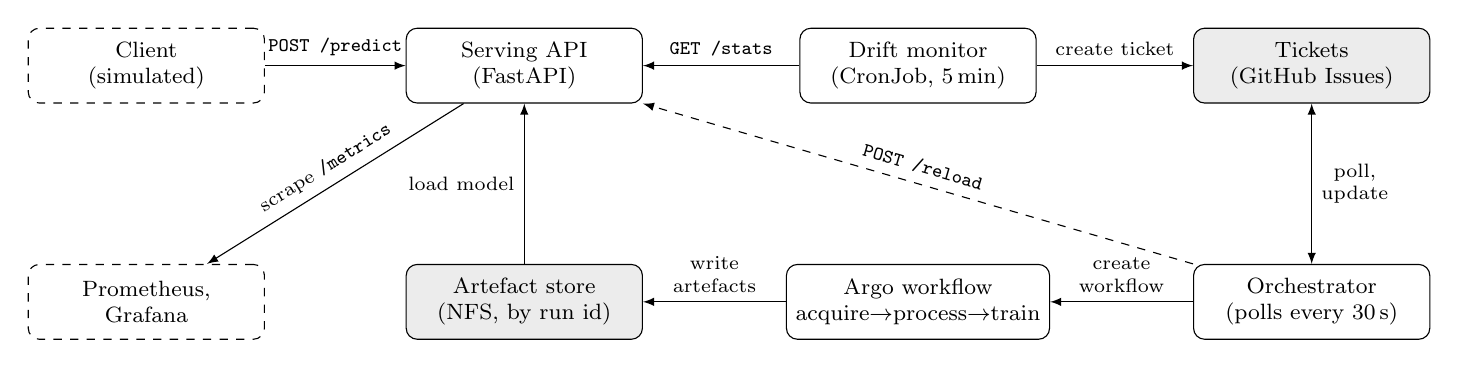
\begin{tikzpicture}[
  box/.style={draw, rounded corners, align=center, minimum height=0.95cm, minimum width=3cm, font=\footnotesize},
  store/.style={box, fill=gray!15},
  ext/.style={box, dashed},
  lbl/.style={font=\scriptsize, align=center}
]
\node[ext]   (client) at (-4.8,0)  {Client\\(simulated)};
\node[box]   (api)    at (0,0)     {Serving API\\(FastAPI)};
\node[box]   (mon)    at (5,0)     {Drift monitor\\(CronJob, 5\,min)};
\node[store] (tix)    at (10,0)    {Tickets\\(GitHub Issues)};
\node[ext]   (obs)    at (-4.8,-3) {Prometheus,\\Grafana};
\node[store] (art)    at (0,-3)    {Artefact store\\(NFS, by run id)};
\node[box]   (wf)     at (5,-3)    {Argo workflow\\acquire$\to$process$\to$train};
\node[box]   (orch)   at (10,-3)   {Orchestrator\\(polls every 30\,s)};

\draw[-latex] (client) -- node[above, lbl]{\texttt{POST /predict}} (api);
\draw[-latex] (mon)    -- node[above, lbl]{\texttt{GET /stats}} (api);
\draw[-latex] (mon)    -- node[above, lbl]{create ticket} (tix);
\draw[latex-latex] (tix) -- node[right, lbl]{poll,\\update} (orch);
\draw[-latex] (orch)   -- node[above, lbl]{create\\workflow} (wf);
\draw[-latex] (wf)     -- node[above, lbl]{write\\artefacts} (art);
\draw[-latex] (art)    -- node[left, lbl]{load model} (api);
\draw[-latex, dashed] (orch.north west) -- node[above, sloped, lbl]{\texttt{POST /reload}} (api.south east);
\draw[-latex] (api)    -- node[above, sloped, lbl]{scrape \texttt{/metrics}} (obs);
\end{tikzpicture}}
\caption{Architecture of the PoC. The monitor also reads the reference statistics from the artefact store and pushes its metrics to a Pushgateway (not drawn).}
\label{fig:poc-arch}
\end{figure}

\subsection{Experimental scenario}

The scenario script runs five steps against the live cluster and logs each of them with a timestamp:
(1)~run the baseline workflow (run identifier \texttt{baseline-001}, no shift) and reload the API;
(2)~send 200 \texttt{/predict} requests drawn from the reference distribution and check that no drift is reported;
(3)~send 200 requests whose six features are shifted by 1.5 reference standard deviations and wait for the monitor to create a ticket;
(4)~wait for the orchestrator to retrain, close the ticket and for the API to serve the new model;
(5)~send the shifted data again and check that the new model's reference no longer reports drift.

The drift rule follows the paper's idea of a runtime check, with parameters we chose: for each feature, $z = |\bar{x}_{\text{now}} - \mu_{\text{ref}}| / \sigma_{\text{ref}}$, where $\bar{x}_{\text{now}}$ is the mean over the last 200 requests; drift is declared when at least three features have $z > 1.0$ and the window holds at least 100 requests.
The monitor runs every five minutes and the orchestrator polls the tickets every 30 seconds.
Retraining uses a shift of 1.5 standard deviations, so the new reference matches the shifted data.

\subsection{Results}

Table~\ref{tab:poc-results} reports the run; every value can be traced to the log file \texttt{scenario/logs/20261015T121211Z.md} (start 12:06:20Z, end 12:12:11Z, total 5\,min\,51\,s). All five steps passed.

\begin{table}[t]
\centering
\caption{Result of the end-to-end run (source: \texttt{scenario/logs/20261015T121211Z.md}).}
\label{tab:poc-results}
\small
\begin{tabularx}{\textwidth}{@{}c >{\raggedright\arraybackslash}p{4.2cm} X l@{}}
\toprule
Step & Expectation & Observation & Outcome \\
\midrule
1 & Baseline workflow succeeds; served model is \texttt{baseline-001} & Workflow succeeded; \texttt{/reload} switched \texttt{issue-6} to \texttt{baseline-001} & Pass \\
2 & $n \geq 100$ and no drift & $n = 200$; largest $z = 0.18$; no feature above 1.0 & Pass \\
3 & \texttt{/stats} shows drift; a \texttt{[drift]} ticket appears & All six features drifted; ticket \#7 created at 12:10:34Z & Pass \\
4 & Ticket closed with label \texttt{done}; served model is \texttt{issue-}\emph{n} & Ticket \#7 closed at 12:12:01Z with labels \texttt{retrain}, \texttt{done}; served model \texttt{issue-7} & Pass \\
5 & No drift against the new model's reference & Model \texttt{issue-7}; $n = 200$; largest $z = 0.13$; no feature above 1.0 & Pass \\
\bottomrule
\end{tabularx}
\end{table}

\paragraph{Timings.}
The shifted requests were sent at 12:07:53Z. The monitor created ticket \#7 at 12:10:34Z (2\,min\,41\,s later, bounded by the five-minute schedule), and the ticket was closed with the new model serving at 12:12:01Z (1\,min\,27\,s after creation). From shifted data to new model took 4\,min\,8\,s.
Across the whole experiment, five ticket-triggered retraining workflows (tickets \#3 to \#7) succeeded, each in 60 to 81 seconds; tickets \#5 and \#7 were created automatically by the monitor, tickets \#3, \#4 and \#6 by hand to test the orchestrator.

\paragraph{Drift evidence.}
At detection, the per-feature $z$ values written in ticket \#7 were 1.44, 1.58, 1.45, 1.46, 1.61 and 1.35 for features \texttt{f0} to \texttt{f5}. After the retraining, the same shifted data gave $z \leq 0.13$ (Table~\ref{tab:poc-results}, step~5). Figure~\ref{fig:poc-grafana} shows the corresponding Grafana dashboard: two drift episodes (largest $z$ about 2.1 and 1.6, six features above the threshold) followed by a return close to zero. Figure~\ref{fig:poc-issue} shows ticket \#7 and Fig.~\ref{fig:poc-argo} the retraining workflow.

\begin{figure}[t]
\centering
\poctryfig{\textwidth}{figures/poc-grafana-6h.png}
\caption{Grafana dashboard over six hours. Top row: served model, drift flag, total predictions, number of drifted features. Middle row: predictions per second by model, prediction latency (p50, p95). Bottom row: largest $z$ with the drift threshold 1.0, and number of drifted features with the threshold 3. Panel titles are in Vietnamese.}
\label{fig:poc-grafana}
\end{figure}

\begin{figure}[t]
\centering
\poctryfig{0.85\textwidth}{figures/poc-issue7-auto.png}
\caption{Ticket \#7, created by the drift monitor and closed by the orchestrator. The text (in Vietnamese) states that the drift was detected automatically by the monitor and lists the per-feature statistics; the second comment, written by the orchestrator, gives the run identifier, accuracy, F1 and the model version after the reload. The account name shown is that of the access token shared by both components.}
\label{fig:poc-issue}
\end{figure}

\begin{figure}[t]
\centering
\poctryfig{0.7\textwidth}{figures/poc-argo-retrain7.png}
\caption{Argo workflow \texttt{retrain-issue-7}: the three steps \texttt{acquire}, \texttt{process} and \texttt{train} completed successfully.}
\label{fig:poc-argo}
\end{figure}

Accuracy and F1 were identical for the baseline and the retrained models (0.915 and 0.916). This is a property of our synthetic data, where the shift translates the whole problem, and not evidence that retraining is useless; we therefore use the disappearance of the drift, not the accuracy, as the evidence for the loop.

\subsection{Observations relevant to the paper's design}

\begin{itemize}
  \item \textbf{Duplicate tickets.} The monitor creates a ticket only if no open ticket labelled \texttt{retrain} exists. Drift persists until the new model is loaded, so without such a rule each five-minute run would open another ticket. This serialises tickets rather than resolving their interaction, a minimal answer to the concurrent-ticket gap that the paper lists.
  \item \textbf{Actor attribution.} The monitor and the orchestrator used one access token, so GitHub attributes every action to the same account. The timeline shows what happened and when, but not which component acted, whereas the paper's audit trail records the acting actor.
  \item \textbf{Detection latency.} Latency has two components: the five-minute schedule and the sliding window. In a local test, 60 shifted requests mixed with 140 earlier ones gave $z$ between 0.3 and 0.6, below the threshold; with a shift of 1.5 standard deviations, roughly two thirds of the window must be shifted before the rule fires.
  \item \textbf{Event versus ticket.} In the paper a component emits an event and the MPO creates the ticket; in the PoC the monitor creates the ticket itself. This removes one hop but also the MPO's role as the single mediator.
  \item \textbf{Idempotence.} Workflow names derive from the ticket number, so a restarted orchestrator finds the existing workflow instead of creating a second one. This was checked with unit tests using fake clients; we did not restart the orchestrator during the live run.
  \item \textbf{Infrastructure.} During installation the control-plane node became unresponsive because the Kubernetes API server exhausted the node's 3.8\,GiB of memory. No instability was observed during the final run, but resource usage was not recorded.
\end{itemize}

\subsection{Differences from the paper and limitations}
\label{sec:poc-diff}

\begin{itemize}
  \item \textbf{No coordination contracts.} The ticket flow is hard-coded; there is no BPMN process and no contract versioning.
  \item \textbf{No human gates.} The plan approval of the paper's scenario (Step~3) is automatic.
  \item \textbf{Collapsed handoffs.} Dataset update and retraining (Steps~4 and~5) run as one workflow under one actor. Step~6 (code update) is never needed because the feature set is fixed; this corresponds to the ``else'' branch of Algorithm~1, but no gate evaluates the input schema.
  \item \textbf{Storage and versioning.} Files and SHA-256 hashes replace MLflow and DVC, which the authors say their own implementation orchestrates; run identifiers replace names such as \texttt{dataset-v3} and \texttt{model-v2.1}; the code version is not recorded in the manifests.
  \item \textbf{Data and model.} Synthetic data and a simple model.
  \item \textbf{One run.} The scenario was executed once, so no variance is available.
  \item \textbf{Scale.} One small cluster, no load or failure testing; this is not a production setting.
\end{itemize}

\subsection{Summary}

The PoC shows that the drift-to-redeployment loop of the paper's scenario can be assembled from off-the-shelf tools and closes in a few minutes on a small cluster, with evidence traceable to a log and to the tickets. It exercises the feedback loop but deliberately omits the coordination contracts, human gates and multi-actor handoffs that distinguish SkeltyMLOps; the claim about coordination therefore remains untested, and the production gap stated by the authors remains open.

% =====================================================================
\section{Conclusion}\label{sec:concl}

Daoud et al.\ address a real gap in MLOps: many tools exist, but there is little architectural guidance on how the actors who build ML-powered software should coordinate. Phase~1 turns a heterogeneous literature into a consolidated vocabulary of five dimensions, five leading actors and 38 activities, using an SLR and a carefully controlled human--LLM consolidation process. Phase~2 shows that existing architectures describe what MLOps involves but leave how actors coordinate largely implicit, and proposes SkeltyMLOps, which puts orchestration and coordination contracts at the centre of the architecture. The methodological transparency of the study is its strongest point. Its main limitation is the evaluation: the architecture is justified by traceability and an illustrative scenario, not by empirical validation or by scoring it against the same benchmark as the baselines. Overall, SkeltyMLOps is a well-grounded reference point for collaborative MLOps. Our scoring (Improvement 1) rates it Yes on four of six criteria and Partial on two, but every cell is a claim drawn from the paper rather than a verified result. Our proof of concept shows that its drift-triggered retraining loop can be assembled from off-the-shelf tools and completes in a few minutes on a small cluster, but it deliberately omits the coordination contracts and human gates that distinguish the design, so the claim about coordination, and its value in production, still have to be demonstrated through a fuller implementation and an industrial evaluation.

% =====================================================================
\begin{thebibliography}{99}

\bibitem{daoud2026} C. Daoud, D. Azar, C. Urtado, and S. Vauttier, ``A reference architecture for an orchestrated collaborative MLOps: A ground-up design from literature combining human and LLM expertise,'' \emph{Future Generation Computer Systems}, vol.~185, p.~108700, 2026. doi: 10.1016/j.future.2026.108700.

\bibitem{daoud2025} C. Daoud, D. Azar, J. Boich\'e, C. Urtado, and S. Vauttier, ``SkeltyMLOps: Orchestrating collaborative MLOps activities,'' in \emph{1st ECAI Workshop on Machine Learning Operations (MLOps25)}, CEUR Workshop Proceedings, vol.~4109, Bologna, Italy, 2025, pp.~55--66.

\bibitem{zenodo} C. Daoud, D. Azar, C. Urtado, and S. Vauttier, ``A reference architecture for an orchestrated collaborative MLOps: A ground-up design from literature combining human and LLM expertise'' [Dataset], Zenodo, v1.1, 2026. doi: 10.5281/zenodo.21311713.

\bibitem{sculley2015} D. Sculley, G. Holt, D. Golovin, E. Davydov, T. Phillips, D. Ebner, V. Chaudhary, M. Young, J.-F. Crespo, and D. Dennison, ``Hidden technical debt in machine learning systems,'' in \emph{Advances in Neural Information Processing Systems (NeurIPS)}, 2015, pp.~2503--2511.

\bibitem{kreuzberger2023} D. Kreuzberger, N. K\"uhl, and S. Hirschl, ``Machine learning operations (MLOps): Overview, definition, and architecture,'' \emph{IEEE Access}, vol.~11, pp.~31866--31879, 2023. doi: 10.1109/ACCESS.2023.3262138.

\bibitem{najafabadi2024} F. A. Najafabadi, J. Bogner, I. Gerostathopoulos, and P. Lago, ``An analysis of MLOps architectures: A systematic mapping study,'' in \emph{Software Architecture -- 18th European Conference (ECSA)}, LNCS vol.~14889, Springer, 2024, pp.~69--85.

\bibitem{eken2025} B. Eken, S. Pallewatta, N. K. Tran, A. Tosun, and M. A. Babar, ``A multivocal review of MLOps practices, challenges and open issues,'' \emph{ACM Computing Surveys}, vol.~58, no.~2, pp.~39:1--39:35, 2025.

\bibitem{wozniak2025} A. P. Wo\'zniak, M. Milczarek, and J. Wo\'zniak, ``MLOps components, tools, process, and metrics -- A systematic literature review,'' \emph{IEEE Access}, vol.~13, pp.~22166--22175, 2025.

\bibitem{kitchenham2007} B. A. Kitchenham and S. Charters, ``Guidelines for performing systematic literature reviews in software engineering,'' Version 2.3, Tech. Rep. EBSE-2007-01, Keele University, 2007.

\bibitem{rodrigues2025} M. G. Rodrigues, E. K. Viegas, A. O. Santin, and F. Enembreck, ``A MLOps architecture for near real-time distributed stream learning operation deployment,'' \emph{Journal of Network and Computer Applications}, vol.~238, p.~104169, 2025.

\bibitem{burgueno2025} A. M. Burgue\~no-Romero, A. Ben\'itez-Hidalgo, C. Barba-Gonz\'alez, and J. F. Aldana-Montes, ``Toward an open source MLOps architecture,'' \emph{IEEE Software}, vol.~42, no.~1, pp.~59--64, 2025.

\bibitem{kumara2025} I. Kumara, R. Arts, R. C. Ferreira, D. Di Nucci, R. Kazman, D. A. Tamburri, and W.-J. van den Heuvel, ``MLOps in practice: Requirements and a reference architecture from industry,'' in \emph{Software Architecture -- 19th European Conference (ECSA)}, LNCS vol.~15929, Springer, 2025, pp.~20--37.

\bibitem{landis1977} J. R. Landis and G. G. Koch, ``The measurement of observer agreement for categorical data,'' \emph{Biometrics}, vol.~33, no.~1, pp.~159--174, 1977.

\end{thebibliography}

\end{document}
